\documentclass[12pt]{article}
\usepackage[margin=1in]{geometry} 
\geometry{letterpaper}   


\usepackage{amssymb,amsfonts,amsmath,bbm,mathrsfs,stmaryrd, mathtools}
\usepackage{xcolor}
\usepackage{url}
\usepackage{dsfont}
\usepackage{enumerate}
\usepackage{enumitem}
\usepackage{MnSymbol,wasysym}
\usepackage{tikz-cd}
\usetikzlibrary{cd}
\usepackage{graphicx}
\graphicspath{ {./images/} }

%\usepackage{parskip}

\usepackage[colorlinks,
             linkcolor=black!75!red,
             citecolor=blue,
             pdftitle={},
             pdfauthor={},
             pdfproducer={pdfLaTeX},
             pdfpagemode=None,
             bookmarksopen=true
             bookmarksnumbered=true]{hyperref}

\usepackage{tikz}
\usetikzlibrary{cd,arrows,calc,decorations.pathreplacing,decorations.markings,intersections,shapes.geometric,through,fit,shapes.symbols,positioning,decorations.pathmorphing}

\usepackage{braket}

\renewcommand{\theequation}{\thesection.\arabic{equation}}

%%%%%%%%%%%%%%%%%%%%%%%%%%%%%%%%
%%% Theorems and references %%%
%%%%%%%%%%%%%%%%%%%%%%%%%%%%%%%%
\usepackage[amsmath,thmmarks,hyperref]{ntheorem}
\usepackage{cleveref}

\creflabelformat{enumi}{#2(#1)#3}

\crefname{section}{Section}{Sections}
\crefformat{section}{#2Section~#1#3} 
\Crefformat{section}{#2Section~#1#3} 

\crefname{subsection}{\S}{\S\S}
\crefformat{subsection}{#2\S#1#3} 
\Crefformat{subsection}{#2\S#1#3} 

\theoremstyle{plain}

\newtheorem{lemma}{Lemma}[section]
\newtheorem{proposition}[lemma]{Proposition}
\newtheorem{corollary}[lemma]{Corollary}
\newtheorem{theorem}[lemma]{Theorem}
\newtheorem{conjecture}[lemma]{Conjecture}
\newtheorem{question}[lemma]{Question}
\newtheorem{assumption}[lemma]{Assumption}


\theoremstyle{nonumberplain}
\newtheorem{theoremN}{Theorem}
\newtheorem{propositionN}{Proposition}
\newtheorem{corollaryN}{Corollary}


\theoremstyle{plain}
\theorembodyfont{\upshape}
\theoremsymbol{\ensuremath{\blacklozenge}}

\newtheorem{definition}[lemma]{Definition}
\newtheorem{example}[lemma]{Example}
\newtheorem{remark}[lemma]{Remark}
\newtheorem{convention}[lemma]{Convention}
\newtheorem{exercise}[lemma]{Exercise}

\crefname{definition}{definition}{definitions}
\crefformat{definition}{#2definition~#1#3} 
\Crefformat{definition}{#2Definition~#1#3} 

\crefname{ex}{example}{examples}
\crefformat{example}{#2example~#1#3} 
\Crefformat{example}{#2Example~#1#3} 

\crefname{remark}{remark}{remarks}
\crefformat{remark}{#2remark~#1#3} 
\Crefformat{remark}{#2Remark~#1#3} 

\crefname{convention}{convention}{conventions}
\crefformat{convention}{#2convention~#1#3} 
\Crefformat{convention}{#2Convention~#1#3} 

\crefname{exercise}{exercise}{exercises}
\crefformat{exercise}{#2exercise~#1#3} 
\Crefformat{exercise}{#2Exercise~#1#3} 



\crefname{lemma}{lemma}{lemmas}
\crefformat{lemma}{#2lemma~#1#3} 
\Crefformat{lemma}{#2Lemma~#1#3} 

\crefname{proposition}{proposition}{propositions}
\crefformat{proposition}{#2proposition~#1#3} 
\Crefformat{proposition}{#2Proposition~#1#3} 

\crefname{corollary}{corollary}{corollaries}
\crefformat{corollary}{#2corollary~#1#3} 
\Crefformat{corollary}{#2Corollary~#1#3} 

\crefname{theorem}{theorem}{theorems}
\crefformat{theorem}{#2theorem~#1#3} 
\Crefformat{theorem}{#2Theorem~#1#3} 

\crefname{assumption}{assumption}{Assumptions}
\crefformat{assumption}{#2assumption~#1#3} 
\Crefformat{assumption}{#2Assumption~#1#3} 

\crefname{equation}{}{}
\crefformat{equation}{(#2#1#3)} 
\Crefformat{equation}{(#2#1#3)}

\theoremstyle{nonumberplain}
\theoremsymbol{\ensuremath{\blacksquare}}

\newtheorem{proof}{Proof.}
\newtheorem{solution}{Solution.}
\newcommand\pf[1]{\newtheorem{#1}{Proof of \Cref{#1}.}}

%%%%%%%%%%%%%%%%%%%%%%%%%%%%%%%%%%%%%%%%%%%%%%%%%%%%%%%%%%%%%
%%%%%%%%%%%%%%%%%%% simple math operators %%%%%%%%%%%%%%%%%%%
%%%%%%%%%%%%%%%%%%%%%%%%%%%%%%%%%%%%%%%%%%%%%%%%%%%%%%%%%%%%%
\DeclareMathOperator{\id}{id}
\DeclareMathOperator{\End}{\mathrm{End}}
\DeclareMathOperator{\pr}{\mathrm{Prob}}
\DeclareMathOperator{\orb}{\mathrm{Orb}}


\DeclareMathOperator{\cact}{\cat{CAct}}
\DeclareMathOperator{\wact}{\cat{WAct}}

%%%%%%%%%%%%%%%%%%%%%%%%%%%%%%%%%%%%%%%%%%%%%%%%%%%%%%%%%%
%%% align* numbering %%%
%%%%%%%%%%%%%%%%%%%%%%%%%%%%%%%%%%%%%%%%%%%%%%%%%%%%%%%%%%

\newcommand\numberthis{\addtocounter{equation}{1}\tag{\theequation}}



%%%%%%%%%%%%%%%%%%%%%%%%%%%%%%%%%%%%%%%%%%%%%%%%%%%%%%%%%%%%
%%%%%%%%%%%%%%%%%%%%%%%%%%%%%%%%%%%%%%%%%%%%%%%%%%%%%%%%%%%%
%%%%%%%%%%%%%%%%%%%%%%%%%%%%%%%%%%%%%%%%%%%%%%%%%%%%%%%%%%%%
%% user macros
%%%%%%%%%%%%%%%%%%%%%%%%%%%%%%%%%%%%%%%%%%%%%%%%%%%%%%%%%%%%
%%%%%%%%%%%%%%%%%%%%%%%%%%%%%%%%%%%%%%%%%%%%%%%%%%%%%%%%%%%%
%%%%%%%%%%%%%%%%%%%%%%%%%%%%%%%%%%%%%%%%%%%%%%%%%%%%%%%%%%%%

% below are many macros
% be careful...

%%%%%%%%%%%%%%%%%%%%%%%%%%%%%%%%%%%%%%%%%%%%%%%%%%%%%%%%%%
%%% misc (should not need to touch) %%%
%%%%%%%%%%%%%%%%%%%%%%%%%%%%%%%%%%%%%%%%%%%%%%%%%%%%%%%%%%

\newcommand\ol{\overline}
\newcommand\wt{\widetilde}

%
\newcommand{\define}[1]{{\em #1}}
\newcommand\1{{\bf 1}}
\newcommand{\cat}[1]{\textsc{#1}}
\newcommand\mathify[2]{\newcommand{#1}{\cat{#2}}}
\newcommand\spr[1]{\cite[\href{https://stacks.math.columbia.edu/tag/#1}{Tag {#1}}]{stacks-project}}
\newcommand{\qedhere}{\mbox{}\hfill\ensuremath{\blacksquare}}


\renewcommand{\square}{\mathrel{\Box}}
\newcommand\Section[1]{\section{#1}\setcounter{lemma}{0}}

%%%%%%%%%%%%%%%%%%%%%%%%%%%%%%%%
%% math fonts
%%%%%%%%%%%%%%%%%%%%%%%%%%%%%%%%


% math blackboard font

\newcommand\bb[1]{{\mathbb #1}} 

\newcommand\bA{{\mathbb A}}
\newcommand\bB{{\mathbb B}}
\newcommand\bC{{\mathbb C}}
\newcommand\bD{{\mathbb D}}
\newcommand\bE{{\mathbb E}}
\newcommand\bF{{\mathbb F}}
\newcommand\bG{{\mathbb G}}
\newcommand\bH{{\mathbb H}}
\newcommand\bI{{\mathbb I}}
\newcommand\bJ{{\mathbb J}}
\newcommand\bK{{\mathbb K}}
\newcommand\bL{{\mathbb L}}
\newcommand\bM{{\mathbb M}}
\newcommand\bN{{\mathbb N}}
\newcommand\bO{{\mathbb O}}
\newcommand\bP{{\mathbb P}}
\newcommand\bQ{{\mathbb Q}}
\newcommand\bR{{\mathbb R}}
\newcommand\bS{{\mathbb S}}
\newcommand\bT{{\mathbb T}}
\newcommand\bU{{\mathbb U}}
\newcommand\bV{{\mathbb V}}
\newcommand\bW{{\mathbb W}}
\newcommand\bX{{\mathbb X}}
\newcommand\bY{{\mathbb Y}}
\newcommand\bZ{{\mathbb Z}}

% math script font

\newcommand\cA{{\mathcal A}}
\newcommand\cB{{\mathcal B}}
\newcommand\cC{{\mathcal C}}
\newcommand\cD{{\mathcal D}}
\newcommand\cE{{\mathcal E}}
\newcommand\cF{{\mathcal F}}
\newcommand\cG{{\mathcal G}}
\newcommand\cH{{\mathcal H}}
\newcommand\cI{{\mathcal I}}
\newcommand\cJ{{\mathcal J}}
\newcommand\cK{{\mathcal K}}
\newcommand\cL{{\mathcal L}}
\newcommand\cM{{\mathcal M}}
\newcommand\cN{{\mathcal N}}
\newcommand\cO{{\mathcal O}}
\newcommand\cP{{\mathcal P}}
\newcommand\cQ{{\mathcal Q}}
\newcommand\cR{{\mathcal R}}
\newcommand\cS{{\mathcal S}}
\newcommand\cT{{\mathcal T}}
\newcommand\cU{{\mathcal U}}
\newcommand\cV{{\mathcal V}}
\newcommand\cW{{\mathcal W}}
\newcommand\cX{{\mathcal X}}
\newcommand\cY{{\mathcal Y}}
\newcommand\cZ{{\mathcal Z}}

% math frak font

\newcommand\fA{{\mathfrak A}}
\newcommand\fB{{\mathfrak B}}
\newcommand\fC{{\mathfrak C}}
\newcommand\fD{{\mathfrak D}}
\newcommand\fE{{\mathfrak E}}
\newcommand\fF{{\mathfrak F}}
\newcommand\fG{{\mathfrak G}}
\newcommand\fH{{\mathfrak H}}
\newcommand\fI{{\mathfrak I}}
\newcommand\fJ{{\mathfrak J}}
\newcommand\fK{{\mathfrak K}}
\newcommand\fL{{\mathfrak L}}
\newcommand\fM{{\mathfrak M}}
\newcommand\fN{{\mathfrak N}}
\newcommand\fO{{\mathfrak O}}
\newcommand\fP{{\mathfrak P}}
\newcommand\fQ{{\mathfrak Q}}
\newcommand\fR{{\mathfrak R}}
\newcommand\fS{{\mathfrak S}}
\newcommand\fT{{\mathfrak T}}
\newcommand\fU{{\mathfrak U}}
\newcommand\fV{{\mathfrak V}}
\newcommand\fW{{\mathfrak W}}
\newcommand\fX{{\mathfrak X}}
\newcommand\fY{{\mathfrak Y}}
\newcommand\fZ{{\mathfrak Z}}

\newcommand\fa{{\mathfrak a}}
\newcommand\fb{{\mathfrak b}}
\newcommand\fc{{\mathfrak c}}
\newcommand\fd{{\mathfrak d}}
\newcommand\fe{{\mathfrak e}}
\newcommand\ff{{\mathfrak f}}
\newcommand\fg{{\mathfrak g}}
\newcommand\fh{{\mathfrak h}}
%\newcommand\fi{{\mathfrak i}}
\newcommand\fj{{\mathfrak j}}
\newcommand\fk{{\mathfrak k}}
\newcommand\fl{{\mathfrak l}}
\newcommand\fm{{\mathfrak m}}
\newcommand\fn{{\mathfrak n}}
\newcommand\fo{{\mathfrak o}}
\newcommand\fp{{\mathfrak p}}
\newcommand\fq{{\mathfrak q}}
\newcommand\fr{{\mathfrak r}}
\newcommand\fs{{\mathfrak s}}
\newcommand\ft{{\mathfrak t}}
\newcommand\fu{{\mathfrak u}}
\newcommand\fv{{\mathfrak v}}
\newcommand\fw{{\mathfrak w}}
\newcommand\fx{{\mathfrak x}}
\newcommand\fy{{\mathfrak y}}
\newcommand\fz{{\mathfrak z}}


\newcommand\fgl{\mathfrak{gl}}
\newcommand\fsl{\mathfrak{sl}}
\newcommand\fsp{\mathfrak{sp}}


%%%%%%%%%%%%%%%%%%%%%%%%%%%%%%%%%%%%%%%%%%%%%%%%%%%%%%%%%%
%%% QIT useful commands %%%
%%%%%%%%%%%%%%%%%%%%%%%%%%%%%%%%%%%%%%%%%%%%%%%%%%%%%%%%%%

\newcommand{\bmat}[1]{\begin{bmatrix*} #1 \end{bmatrix*}} % matrices
\newcommand{\setovecs}[1]{\lb \ket{v_1}, \ldots, \ket{v_{#1}}\rb} % set of vectors
\newcommand{\listovecs}[2]{\ket{{#1}_1}, \ldots, \ket{{#1}_{#2}}} % set list of NAMED vectors
\newcommand{\Tr}{\text{Tr}} % trace v1
\newcommand{\tr}{\text{tr}} % trace v2

%%%%%%%%%%%%%%%%%%%%%%%%%%%%%%%%%%%%%%%%%%%%%%%%%%%%%%%%%%
%%% standard mitch commands %%%
%%%%%%%%%%%%%%%%%%%%%%%%%%%%%%%%%%%%%%%%%%%%%%%%%%%%%%%%%%

%% Standard Sets
\newcommand{\Q}{\mathbb{Q}} % rationals
\newcommand{\R}{\mathbb{R}} % reals
\newcommand{\Z}{\mathbb{Z}} % integers
\newcommand{\C}{\mathbb{C}} % complex numbers
\newcommand{\N}{\mathbb{N}} % natural numbers
\newcommand{\F}{\mathbb{F}} % arbitrary field
\newcommand{\T}{\mathbb{T}} % Unit circle
\newcommand{\D}{\mathbb{D}} % Open unit disc

%% Arrows
\newcommand{\ra}{\rightarrow}
\newcommand{\Ra}{\Rightarrow}
\newcommand{\La}{\Leftarrow}

%% Greek
\newcommand{\al}{\alpha}
\newcommand{\ep}{\varepsilon} % epsilon
\newcommand{\es}{\varnothing} % empty set


%% Brackets
\newcommand{\<}{\left\langle} 
\renewcommand{\>}{\right\rangle}
\newcommand{\lp}{\left(}
\newcommand{\rp}{\right)}
\newcommand{\lv}{\left\lvert}
\newcommand{\rv}{\right\rvert}
\newcommand{\lb}{\left\{}
\newcommand{\rb}{\right\}}
\newcommand{\lan}{\left\langle}
\newcommand{\ran}{\right\rangle}

%% Algebra
\newcommand{\isom}{\cong} %Isomorphic
\newcommand{\nsub}{\trianglelefteq} %Normal Subgroup
\newcommand{\semi}{\rtimes} %Semi-Direct Product
\newcommand{\Aut}{\text{Aut}} % automorphism group
\newcommand{\op}{{\text{op}}} % opposite algebra

%% Linear Algebra
\newcommand{\norm}[1]{\left\lVert#1\right\rVert} % norm
\newcommand{\inp}[2]{\left\langle#1, #2\right\rangle} % inner product
\newcommand{\spn}[1]{\text{Span}\lp #1\rp} % span
\newcommand{\cspn}[1]{\overline{\text{Span}}\lp #1\rp} % closed span

%% Analysis
\newcommand{\abs}[1]{\left\lvert #1 \right\rvert} % absolute value
\newcommand{\supp}[1]{\text{supp}\lp #1\rp} % support
\newcommand{\co}{\text{co}} % convex hull
\newcommand{\cl}[1]{\overline{#1}} % closure
\DeclareMathOperator*{\esssup}{ess\,sup} % essential supremum

%% Complex 
\newcommand{\Res}[2]{\text{Res}\lp #1, #2\rp} %Residue of a FUNCTION at a POINT
\newcommand{\Ind}{\text{Ind}} % index
\newcommand{\re}[1]{\text{Re}(#1)}  % real part
\newcommand{\im}[1]{\text{Im}(#1)} % complex part

%% XPatch
\usepackage{xpatch}
\xpatchcmd{\qed}{\hfill}{}{}{}
%%%%%%%%%%%%%%%%%%%%%%%%%%%%%%%%
%%% ACTUAL PREAMBLE %%%
%%%%%%%%%%%%%%%%%%%%%%%%%%%%%%%%

\title{Introduction to Quantum Information Theory}
\author{Joshua Parmenter}
\date{19 Jan, 2021}


\begin{document}

\maketitle

\begin{abstract}
Quantum Information is a field that is becoming more and more relevant as computers get faster and more intelligent.  This document is designed to be a fast paced, rapid introduction to the concepts necessary to comprehend the math and theories behind the creation, editing, and analysis of quantum bits, especially with a focus on sending and receiving information, or processing large or mathematically intensive computations. 
\end{abstract}

\tableofcontents
\pagebreak
%%%%%%%%%%%%%%%%%%%%%%%%%%%%%%%%%%%%%%%%%%%%%%%%%%%%%%%%%
%%%%%%%%%%%%%%%%%%%%%%%%%%%%%%%%%%%%%%%%%%%%%%%%%%%%%%%%%
% Where the work happens...
%%%%%%%%%%%%%%%%%%%%%%%%%%%%%%%%%%%%%%%%%%%%%%%%%%%%%%%%%
%%%%%%%%%%%%%%%%%%%%%%%%%%%%%%%%%%%%%%%%%%%%%%%%%%%%%%%%%

%%%%%%%%%%%%%%%%%%%%%%%%%%%%%%%%%%%%%%%%%%%%%%%%%%%%%%%%%
%%%%%%%%%%%%%%%%%%%%%%%%%%%%%%%%%%%%%%%%%%%%%%%%%%%%%%%%%
\section{Vectors and Vector Spaces}
%%%%%%%%%%%%%%%%%%%%%%%%%%%%%%%%%%%%%%%%%%%%%%%%%%%%%%%%%
%%%%%%%%%%%%%%%%%%%%%%%%%%%%%%%%%%%%%%%%%%%%%%%%%%%%%%%%%

\subsection{Vector Spaces}
In modern mathematics, an area of importance is first defining what field the problems are being asked in.  When speaking on vectors and vector spaces, it is easiest to work in two main fields of numbers.

\subsubsection{Relevant Vector Spaces}
\begin{enumerate}
	\item $\R$ : \textbf{All Real Numbers} $(\infty, -\infty)$ \\
	
	This includes all real numbers from zero to infinity, something of note is that this number field is \textbf{not algebraically closed}, meaning not all numbers can be produced from combinations of other numbers in the field.  An example of this is $x^2 + 1 = 0$, meaning $x = 1*i$
	
	\item $\C$ : \textbf{All Complex Numbers} \\
	
	This number field \textbf{is algebraically closed}.  This means that every possible number in the field can be produced from combinations of other numbers in the field.  This makes sense as two complex numbers multiplied together can produce 1. A completely real number 2. A complex number with a real and imaginary component 3. A complex number with only an imaginary component.
\end{enumerate}

\subsection{Complex Number Operations}
\textit{In the following sections, we will make the assumption $a, b, c, d, e \in \R$}
	\subsubsection{Addition}	
\begin{equation}
(a + bi) + (c + di) = (a+c) + (b+d)i 
\end{equation}

\subsubsection{Multiplication}	
\begin{equation}
(a+bi) * (c + di) = (ac+adi) + (bci-bd)
\end{equation}

\subsubsection{Conjugation}	
\begin{equation}
\overline{a + bi} = (a + bi)^* = a - bi
\end{equation}

\subsubsection{Modulus}	
\begin{equation}
|z| = |a + bi| = \sqrt[]{a^2 + b^2} 
\end{equation}
		
	
		
\subsection{Common Vector Space Notation and Definitions}
This section is to lay out some of the most important pieces of notation and definitions for the complex mathematics required for this course.  
\subsubsection{Linear Algebra Terms}
\begin{definition}
An element $\ket{v}\in \C^n$ is called a \textbf{(ket) vector} and is expressed as a \textbf{column} of $n$ complex numbers. The integer $n$ is called the \textbf{dimension} of the vector space $\C^n.$
\end{definition}

\begin{definition}
A \textbf{linear combination} of ${\ket{v_1}, ... , \ket{v_k}} \subset \C^n$ is just a single vector in the form $\lambda_1\ket{v_1} + \lambda_2\ket{v_2} + ... + \lambda_k\ket{v_k}$ for some $\lambda_1, \lambda_2, ..., \lambda_k  \in \C$.
\label{def:Combination}
\end{definition}


\begin{example}
Create a \textbf{linear combination} of $\ket{v_1} = \bmat{i\\1}$, $\ket{v_2} = \bmat{-1\\i + 1}$\\
To create a linear combination, we simply must add two complex number constants $\lambda_1, \lambda_2$ in the form shown in  \hyperref[def:Combination]{Definition 1.2}, $\mathbf{\lambda_1\ket{v_1} + \lambda_2\ket{v_2}}$. \\
\begin{equation*} 
\begin{split}
\lambda_{final}\ket{v_{final}} = \lambda_1\ket{v_1} + \lambda_2\ket{v_2} \qquad\qquad    
&\lambda_1 = 1\\
&\lambda_2 = 3 + 2i
\end{split}
\end{equation*}\\

\begin{equation}
\begin{split}
\lambda_{final}\ket{v_{final}} & = 1\bmat{i\\ 1} + (3 + 2i) \bmat{-1\\ i + 1}\\
& = \bmat{i\\ 1} + \bmat{-3 - 2i\\ 1 + 5i}\\
& = \bmat{-3 - i\\ 3 + 5i}
\end{split} 
\end{equation}
\end{example}

\begin{definition}
\label{def:Independence}
Two vectors $\ket{v_1}, \ket{v_2}$ are \textbf{linearly independent} if the only way to create the 0 vector from a linear combination is through setting all complex constants $\lambda_1, \lambda_2, ... , \lambda_k$ to zero in the linear combination formula described in \hyperref[def:Combination]{Definition 1.2}.
\end{definition}

\begin{definition}
A \textbf{subspace} of complex plane $\C$ is a set $\mathbf{M} \in \C^n$ that satisfies three properties:
\begin{itemize}
\item $\ket{0} \in \mathbf{M}$
\item $\ket{v} + \ket{u} \in  \mathbf{M}$ for all $\ket{v}, \ket{u}$
\item $c\ket{v} \in \mathbf{M}\;\; \forall\;\; \ket{v} \in \mathbf{M},\; c \in \C$
\end{itemize}   
\end{definition}

\begin{definition}
The \textbf{span} of a set \textbf{S} is the smallest linear subspace $\in$ \textbf{S}.  
\end{definition}

\begin{theorem}
\textbf{(Span of a set is always a subspace theorem)}\\
Let $\mathbf{s} = \{ \ket{v_1}, \ket{v_2}, ... , \ket{v_k} \} \subset \C^n$, then $span(\mathbf{s})$ is a subspace of $\C^n$
\\
\begin{proof} \renewcommand{\qedsymbol}{}
\begin{enumerate}
\item Note that $\ket{0} = 0\ket{v_1} + 0\ket{v_2}  + ... + 0\ket{v_k} \in span(\mathbf{s})$. 
\item Let $\ket{v}, \ket{u} \in span(\mathbf{s})$ be arbitrary. \\
\\ 
Since  $\ket{v}, \ket{u} \in span(\mathbf{s})$, there exists scalars $c_1, c_2, ... , c_k$ and $d_1, d_2, ... , d_k$ such that 
\begin{align*}
\ket{v} = &c_1\ket{v_1}, ... ,  c_k\ket{v_k} \\
\ket{u} = &d_1\ket{v_1}, ... ,  d_k\ket{v_k}
\end{align*}

then, 
\begin{align*}
\ket{v} + \ket{u} &= (c_1\ket{v_1}, ... ,  c_k\ket{v_k}) +   d_1\ket{u_1}, ... ,  d_k\ket{u_k}\\
 &= (c_1 + d_1)\ket{v_1} + ... + (c_k + d_k)\ket{v_k}\; \in\; span(\mathbf{s})
\end{align*}
This is the true because all of these are linear combinations consisting of a complex constant and a ket vector, which coincides with the \hyperref[def:Combination]{Linear Combination Definition 1.2}.\\
\item Let $\ket{w} \in span(\mathbf{s})$ and $c \in \C$.
If this is true, then there exists $\lambda_1, \lambda_2, ... , \lambda_k$ such that $\ket{v} = \lambda_1\ket{v_1}, ... ,  \lambda_k\ket{v_k}$.  Consider: 
\begin{equation} 
\begin{split}
c\ket{w} &= c\ket{v} \\
&= C(\lambda_1\ket{v_1}, ... ,  \lambda_k\ket{v_k}) \\
&= (C\lambda_1)\ket{v_1} + ... + (C\lambda_k)\ket{v_k}
\end{split}
\end{equation}
\textbf{Equation 1.6} shows that after distributing \textbf{C} in, we have another linear combination, which must exist inside of $span(\mathbf{s})$, and since $span(\mathbf{s})$ satisfies 1,2,3, $span(\mathbf{s})$ must be a subspace.
\end{enumerate}
\end{proof}
\end{theorem}

\begin{theorem}
\textbf{Basis Theorem} \\
If \textbf{S} is a set of \textbf{n} linearly independent vectors in $\C^\mathbf{n}$, then $span(\mathbf{S}) = \C$.
\end{theorem}

\begin{definition}
A \textbf{basis} of a subspace $M \subseteq \C^n$ is a set of vectors \textbf{S} such that 
\begin{enumerate}
\item S is linearly independent.
\item $span(\mathbf{S}) = M$, or in plain English "S spans M"
\end{enumerate}
\end{definition}

\begin{definition}
The \textbf{dimension} of a space is the number of vectors in it. 
\end{definition}

\begin{example}
\textbf{Standard basis of different complex vector spaces.}\\ 
\\
\begin{itemize}
\item Standard Basis for $\C^2$: $\bmat{1\\ 0}, \bmat{0\\ 1}$
\item Standard Basis for  $\C^n$: $\bmat{1\\ 0\\ \vdots\\ 0}, \bmat{0\\ 1\\ \vdots\\ 0}, ... , \bmat{0\\ 0\\ \vdots\\ 1}$
\end{itemize}
\end{example}

\begin{exercise}[Vector Space Exercise]
Below are some exercises designed to put the concepts in this section to work, in order to further reinforce learning.
\begin{enumerate}
\item Consider S = $\{\ket{v_1},\ket{v_2},\ket{v_3}\}$, where $\ket{v_1} = \bmat{1\\ -1}, \ket{v_2} = \bmat{i\\ 1}, \ket{v_3} = \bmat{0\\ i}$
	\begin{enumerate}
	\item Give a linear combination of the vectors in S.\\
	\begin{equation}
	\lambda\ket{v} = 1\bmat{1\\ -1} + 1\bmat{i\\ 1} - (1 + 200i)\bmat{0\\ i}
	\end{equation}
	\item Determine if $\bmat{1 + i\\ 200 - i}$ is in Span($S$).
	\begin{equation*}
	\begin{split}
		\alpha\ket{v1} + \beta\ket{v_2} + \gamma\ket{v_3} &= \bmat{1 + i\\ 200 - i},\qquad 	\alpha = 1, \beta = 1, \gamma = ?\\
		1\bmat{1\\ -1} + 1\bmat{i\\ 1} - \gamma\bmat{0\\ i} &= \bmat{1 + i\\ 200 - i}				\text{Choose alpha and beta to obtain} \bmat{1+i\\ 0}\\
		\bmat{1 + i\\ 0} - \gamma\bmat{0\\ i} &= \bmat{1 + i\\ 200 - i}\qquad \text{Now we must isolate $\gamma$}\\
		\bmat{0\\ \gamma*i} &= \bmat{0\\ -200 + i}\qquad \text{We now set the matrix as an equality}\\
		\gamma*i &= -200+i\\
		\gamma &= -(1 + 200i)\\
		1\bmat{1\\ -1} + 1\bmat{i\\ 1} - (1 + 200i)\bmat{0\\ i} &= \bmat{1 + i\\ 200 - i} 
	\end{split}
	\end{equation*} 
	Since we were able to create a linear combination of the vectors that satisfy the given vector, it is in Span($S$).
	\item Describe Span($S$) geometrically. \\
	\\
	Span($S$) is every possible vector $\in \C^2$
	\end{enumerate}
\end{enumerate}
\end{exercise}

\pagebreak

\begin{exercise} [Linear Independence Exercise]
Find the condition under which the following two vectors are linearly independent.\\
\begin{equation*}
\ket{v_1} = \bmat{x\\ y\\ 3} \in \R,\qquad \ket{v_2} = \bmat{2\\ x - y\\ 1} \in \R
\end{equation*}

\begin{equation}
\begin{split}
	\bmat{x\\ y\\ 3} = \alpha\bmat{2\\ x-y\\ 1}\\
\end{split}
\end{equation}
\text{First, we must  make this linearly dependent so we know when x and y fail linear independence}\\
\begin{equation*}
\begin{split}
	\alpha = 3 \quad \rightarrow \quad \bmat{x\\ y\\ 3} &= 3\bmat{2\\ x-y\\ 1}\\
	\bmat{x\\ y\\ 3} &= \bmat{6\\ 3(x-y)\\ 3}\\ 
\end{split}
\end{equation*}
\begin{center}
Now we need to make this an equality to solve for x and y.
\end{center}
\begin{equation*}
\begin{split}
	x = 6 \quad \rightarrow \quad y &= 3(x-y)\\
	y &= 3x - 3y\\
	4y &= 18\\
	y &= 9/2 \text{(or 4.5)}
\end{split}
\end{equation*}
\end{exercise}

\pagebreak

\begin{exercise} [Basis Exercise]
Show that the set formed by the following vectors is a basis for $C^3$\\
\begin{center}$
\ket{V_1} = \bmat{1\\ 1\\ 1},\; \ket{V_1} = \bmat{1\\ 0\\ 1},\; \ket{V_1} = \bmat{1\\ -1\\ -1}\; 
$\\
\end{center}
There are two things we must prove in order for a set of vectors to form a basis: linear independence and an equal number of vectors as the dimension of the space.\\
First we will prove linear independence:\\\\
\textbf{1. Linear Independence Test}
\begin{equation}
\begin{split}
	&\bmat{1& 1& 1& 0\\ 1& 0& -1& 0\\ 1& 1& -1& 0} \text{First, we build augmented matrix}\\
	\xrightarrow{R_2 - R_3} &\bmat{1& 1& 1& 0\\ 0& -1& 0& 0\\ 1& 1& -1& 0}\\
	\xrightarrow{R_3 - R_1} &\bmat{1& 1& 1& 0\\ 0& -1& 0& 0\\ 0& 0& -2& 0}\\
	\xrightarrow{-1*R_2,\;-\tfrac{1}{2}*R_3} &\bmat{1& 1& 1& 0\\ 0& 1& 0& 0\\ 0& 0& 1& 0}\\
	\xrightarrow[R_1 - R_3]{R_1 - R_2} &\bmat{1& 0& 0& 0\\ 0& 1& 0& 0\\ 0& 0& 1& 0}\\ 
\end{split}
\end{equation}
Thus, we have proved that if the only way to obtain the [0] matrix is through $\lambda_1, ... , \lambda_k = 0$ as mentioned in \hyperref[def:Independence]{Definition 1.4}, we know that the vectors are \textbf{linearly independent}.\\ 
\\
\textbf{2. Dimension Test}
\\\\
Now we must prove that the dimension of the space is equal to the number of the vectors, and since we are working with $C^3$ and we have $\ket{V_1}, \ket{V_2}, \ket{V_3}$ we know that our space has three dimensions and we have three vectors, therefore we have just proven that \textbf{the given set of vectors forms a basis for $\mathbf{\C^3}$.}
\end{exercise}
\pagebreak
\subsection{Inner/Outer Products, and Norms of Vectors}
\begin{definition}
The \textbf{dual space of $\mathbf{\C^n}$} ($\mathbf{\C^{n^*}}$) is a space of row vectors where there are n entries from $\C$. 
\end{definition}
\begin{definition}
A \textbf{transpose} is an operation that every column into a row vector and vice versa without changing the order.
\end{definition}
\begin{example}[Example of transpose operation]
\begin{equation}
\ket{V}^\dagger = \bmat{7\\ 8i\\ \pi+3i\\ 0}^\dagger
\end{equation}
\begin{equation}
\bra{V} = \bmat{7& 8i& \pi+3i& 0}
\end{equation}
It can be seen that the only difference between \textbf{1.10} and \textbf{1.11} is that we have converted the column to a row, this is accomplished through the \textbf{dagger ($\mathbf{\dagger)}$} being applied to a matrix or vector.
\end{example}

\begin{definition}
Given $\ket{V}, \ket{W}$, the \textbf{inner product} of $\ket{V}, \ket{W}$ is $\braket{W|V}$ which can also be written as ${\bra{W}} * \ket{V}$. \\ \textit{It should be noted that the inner product of a bra and ket vector will always yield a constant}.
\end{definition}

\begin{example}[Example of an Inner Product on $\R^n$]
\begin{equation}
\ket{V} = \bmat{1\\ 1\\ 3}, \ket{W} = \bmat{5\\ -2\\ 1}
\end{equation}
\begin{equation}
\braket{W|V} = \bmat{5& -2& 1}\bmat{1\\ 1\\ 3} = 5 - 2 + 3 = 6
\end{equation}
\textit{It should be noted that the inner product on $\R^n$ is just the usual dot product.}
\end{example}

\begin{example}[Example of an Inner Product on $\C^n$]
\begin{equation}
\ket{V} = \bmat{i\\ 1}, \ket{W} = \bmat{-i\\ -1}
\end{equation}
\begin{equation}
\braket{W|V} = \bmat{-i& -1}\bmat{i\\ 1} = 1 - 1 = \mathbf{0} 
\end{equation}
\textit{The inner product yielding 0 means that the two vectors are \textbf{orthogonal}.}
\end{example}

\pagebreak
\begin{definition}
The \textbf{norm (or magnitude)} of $\ket{V} \in \C^n$ is 
\begin{equation}
\norm{\ket{V}} \coloneqq \sqrt{\braket{V|V}}
\end{equation}
\end{definition}

\begin{example} [Example of taking the norm of a complex vector]
\begin{equation*}
\begin{split}
v &= \bmat{1,1} \in \R^2\\
\norm{\ket{V}} &\coloneqq \sqrt{\bmat{1 & 1}|\bmat{1\\ 1}} = \sqrt{1+1} = \sqrt{2}
\end{split}
\end{equation*}
\textbf{Two points of note:}\\
1. Can $\braket{W|V}$ be complex?\qquad\qquad\;         \textbf{YES}\\
2. Can $\braket{V|V}$ = $\norm{\ket{V}}^2 \in \C?$\qquad\qquad   \textbf{YES}
\end{example}

\begin{definition}
A set of nonzero vectors S = $\{\ket{V_1}, \ket{V_2}, ... , \ket{V_k}\} \leq \C^n$ is called \textbf{an orthogonal set} if $\mathbf{\braket{v_i|v_j} = 0}$ if $\mathbf{i \neq j}$.
\end{definition}

\begin{theorem} [Orthogonality and Linear Independence Theorem]  
In this theorem, we will use what we have learned so far in order to gain a deeper understanding into the properties of orthogonality in a vector space.\\ \\
\textbf{If S = {$\ket{V_1}, ... , \ket{V_1}$} is an orthogonal vector set of nonzero vectors in $\C^n$, then S is linearly independent. } 
\begin{proof}  \renewcommand{\qedsymbol}{}
Let $c_1, ... , c_k \in \C$ s.t. $c_1\ket{v_1}, c_2\ket{v_2}, ... , c_k\ket{v_k} = \ket{0}$.
\\
\textbf{Goal}: Show $c_1, ... , c_k = 0$ using assumption S is orthogonal set.\\
\\
Let $j \in \{1, ... , k\}$, then 
\begin{equation}
\begin{split}
&\bra{v_j}(c_1\ket{v_1}, ... , c_k\ket{v_k}) = \braket{v_j|0}\\
&c_1\braket{v_j|v_1}+ ... + c_k\braket{v_j|v_k}\\
&c_j\braket{v_j|v_j} = \text{Since S is an orthogonal set}
\end{split}
\end{equation}
Since $\braket{v_j|v_j}$ can't possibly be 0 because we know that $j \neq 0$, it means that $c_k$ must be zero, which as stated in the \hyperref[def:Independence]{Linear Independence Definition}, means that S is linearly independent.  
\end{proof}
\end{theorem}

\begin{definition}
A basis is \textbf{orthonormal} if two conditions are satisfied: 
\begin{enumerate} \renewcommand{\blacklozenge}{}
\item S is an orthogonal set of \textit{n} unit vectors.
\item Span(S) $\in \C^n$
\end{enumerate} 
In plain English, an orthonormal basis is a basis in which there are exactly the number of vectors as the dimension of the space (from the basis definition) as well as well as all of those vectors being orthogonal to each other.  
\end{definition}

\pagebreak

\begin{exercise}  [Basis Practice]  In this example, there will be multiple transformations completed to gain a better understanding of what a basis is, and what it means to be orthogonal. \leavevmode\linebreak  
\begin{enumerate}
\item 
\begin{equation} \renewcommand{\blacklozenge}{}
\ket{b_1} = \frac{1}{\sqrt{2}}\bmat{1\\ 1} \qquad\qquad \ket{b_2} = \frac{1}{\sqrt{2}}\bmat{1\\ -1}
\end{equation}
	\begin{enumerate}
	\item Show that $\mathcal{B}$ is an orthonormal basis for $\C^2$.\\
		\begin{enumerate}
		\item Check orthogonality:\\
		\begin{equation*}
		\braket{b_1|b_2} = \frac{1}{\sqrt{2}}(\bmat{1 & 1}\bmat{1\\ -1} = 1 - 1 = \mathbf{0}
		\end{equation*}
		These two vectors are orthogonal since their inner product is 0. \\
		\item Check that they are unit vectors: (is the norm one?) \\
		\begin{equation*}
		\begin{split}
		\norm{\ket{b_1}} = \sqrt{\braket{b_1|b_1}} = \frac{1}{\sqrt{2}}\sqrt{1+1} = \frac{\sqrt{2}}{\sqrt{2}} = &\mathbf{1}\\
		\norm{\ket{b_2}} = \sqrt{\braket{b_2|b_2}} = \frac{1}{\sqrt{2}}\sqrt{1^2+(-1)^2} = \frac{\sqrt{2}}{\sqrt{2}} = &\mathbf{1}
		\end{split}
		\end{equation*}
		\end{enumerate}
		This means that, since the vectors are orthogonal and unit vectors, they are orthonormal, forming an orthonormal basis for $\C^2$.
	\pagebreak
	\item Find the coordinates of $\ket{x} = \bmat{-2 1}$ relative to basis $\mathcal{B}$ (i.e. find the scalars such that...)
	\begin{equation*}
	\begin{split}
	c_1, c_2 \in \C\; \text{such that}\; c_1\ket{b_1} + c_2\ket{b_2} = \ket{x}\\\\
	\bra{b_1}(c_1\ket{b_1} + c_2\ket{b_2}) = \braket{b_1|x}\\
	c_1\braket{b_1|b_1} + c_2\braket{b_1|b_2} = \braket{b_1|x}\\\\
	\text{$b_1, b_2$ are orthogonal so $\braket{b_1|b_2} = 0$ so}\\\\
	c_1 = \braket{b_1|x}\\
	\boxed{c_1 = \frac{1}{\sqrt{2}} \bmat{1&1}\bmat{-2\\ 1} = \mathbf{\frac{-1}{\sqrt{2}}}}
	\end{split}	
	\end{equation*}
	\begin{equation*}
	\begin{split}
	\bra{b_2}(c_1\ket{b_1} + c_2\ket{b_2}) = \braket{b_2|x}\\
	c_1\braket{b_2|b_1} + c_2\braket{b_2|b_2} = \braket{b_2|x}\\\\
	\text{$b_1, b_2$ are orthogonal so $\braket{b_2|b_1} = 0$ so}\\\\
	c_2 = \braket{b_2|x}\\
	\boxed{c_2 = \frac{1}{\sqrt{2}} \bmat{1&-1}\bmat{-2\\ 1} = \mathbf{\frac{-3}{\sqrt{2}}}}
	\end{split}	
	\end{equation*}
	\end{enumerate}
\end{enumerate}
\end{exercise}
\pagebreak
\begin{definition}
Define $P_i \coloneqq \ket{f_i}\bra{f_i}$ to be the \textbf{projection operator} onto span($\ket{k_i}$)
\end{definition}
\begin{proposition}
Let $\mathcal{B} = \{\ket{f_1}, ... , \ket{f_n}\}$ be an orthonormal basis for $\C^n$ then...\\
\begin{enumerate}
\item $P_i(\ket{v}) \in span(\ket{f_1}) $
\item $\ket{v} - P_i\ket{v}$ is orthogonal to $\ket{f_i}$
\item ${P_i}^2 = P_i * P_i = P_i$ Projection will still be the same.
\item $P_iP_j = 0$ shadow on one plane will be "nothing" in the perspective of another plane.
\item $P_i^\dagger = P_i$ self-adjoint
\item $\sum_{i=1}^{n} P_i = I_n$
\end{enumerate}
\begin{example} [Outer Product Example]
Given $P_2 = \frac{1}{2} \bmat{1 &-1\\ -1& 1}$, what is $P_1 + P_2$\\
\begin{equation*} \renewcommand{\blacklozenge}{}
\begin{split}
P_1 &= \ket{f_1}\bra{f_1}\\
&= \frac{1}{\sqrt{2}} \bmat{1\\1} * \frac{1}{\sqrt{2}}\bmat{1&1}\\
&= \frac{1}{2} \bmat{1&1\\1&1}\\
P_1 + P_2 &= \frac{1}{2} \bmat{1&1\\1&1} + \frac{1}{2} \bmat{1&-1\\-1&1}\\
&= \frac{1}{2} \bmat{0&2\\2&0}\\
&= \bmat{1&0\\0&1}\\
\end{split}
\end{equation*}
This is an interesting result, it shows that if you add all of the projections in a space you will get the identity matrix, proof available elsewhere as I am too lazy to type it out.
\end{example}
\end{proposition}

\textbf{Why is projection useful?}: It allows us to find $c_1, ... , c_k$ for $\ket{x} = c_1\ket{f_1} + ... + c_k\ket{f_k}$  when all $\ket{f}$ are orthogonal to each other.

\pagebreak
\begin{theorem} [The Gram Schmidt Process]
Let {$\ket{b_1}, ... , \ket{b_k}$} be the basis for a subspace M in $\C^n$. Define the set of vectors {$\ket{f_1}, ... , \ket{f_k}$} as follows:\\
\\
\textbf{Step 1:} \\
Define $\ket{f_1} \coloneqq \ket{b_1}$.\\\\
\textbf{Step i+1:} \\
for i = 1:k-1\\
\begin{equation}
\ket{f_{i+1}} \coloneqq \ket{b_{i+1}} - (\sum_{j=1}^{i}  {\frac{\ket{f_j}\bra{f_j}}{\braket{f_j|f_j}}})\ket{b_{i+1}} = \ket{b_{i+1}} - (\sum_{j=1}^{i}  {\frac{\braket{f_j|b_{i+1}}}{\braket{f_j|f_j}}})\ket{f_j}
\end{equation}
\textbf{\textit{Done}}\\\\
\textbf{Now normalization step}\\
for i = 1 : k
\begin{equation}
\ket{f_i} \coloneqq \frac{1}{\norm{\ket{f_i}}}\ket{f_i}
\end{equation}
\textbf{\textit{Done, now we know that $\ket{f_1}, ... \ket{f_k}$ is a orthonormal basis for M}}
\end{theorem}

\textit{A special thank you for Dr. Hamidi and Dr. Ismert for giving this psuedocode function for Gram Schmidt, I have pulled from it heavily in this page as it is the best way to explain this code.}
\pagebreak

\section{Matrices and Linear Transformations}
\subsection{Matrices} \textbf{This section assumes a basic knowledge of matrix operations, and should be a basic overview.}

\begin{definition}
$\mathbf{M_{mn(}\C)}$ = set of all mxn matrices with complex entries.
\end{definition}

\begin{definition}
$\mathbf{M_n(\C) \equiv M_{nn}(\C)}$ meaning that it is just a square matrix with nxn size.  
\end{definition}

\begin{example} [Pauli Matrices]
\begin{equation}
\begin{split}
\sigma_x &= \bmat{0 &1\\ 1 &0}\\
\sigma_y &= \bmat{0 &i\\ -i &0}\qquad\qquad \in M_2\\
\sigma_z &= \bmat{1 &0\\ 0 &-1}\\
\end{split}
\end{equation}
\textit{These three matrices are called the \textbf{Pauli matrices} the the basic matrices we will use for quantum computations in the future.}
\end{example}

\begin{definition}
The \textbf{Identity Matrix} ($I_n$) is the matrix $M_n$ whose columns are the standard basis {$\ket{e_1}, ... , \ket{e_n}$} for $\C_n$.
\begin{equation}
I_4 = \bmat{1 &0 &0 &0\\ 0 &1 &0 &0 \\ 0 &0 &1 &0 \\ 0 &0 &0 &1}
\end{equation}
\end{definition}

\begin{theorem}
$M_n$ has a well defined matrix multiplication, in general, if $A \in M_{mn}, B \in M_{nk}$. \\\\
The matrix $AB = [A\ket{b_1}\;\; ...\;\; A\ket{b_k}]$
\end{theorem}

\begin{example}[Pauli Matrices in action] For this example, we will be scaling the $\sigma_y$ Pauli matrix.
\begin{equation} \renewcommand{\blacklozenge}{•}
\begin{bmatrix}
0 & -i \\
i & 0
\end{bmatrix}\begin{bmatrix}
1 & 0 \\
0 & 3
\end{bmatrix}=\begin{bmatrix}
0 & -3i \\
i & 0
\end{bmatrix}=\bmat{1\ket{a_1} &3\ket{a_2}}
\end{equation}
This shows that in general, multiplying a row matrix by a diagonal matrix will scale the row matrix by the respective diagonal matrix value.
\end{example}

\pagebreak

\subsection{Eigenvectors and Eigenvalues}

\subsubsection{Eigenvalues/Eigenvectors}

\begin{definition}
An \textbf{eigenvalue} for $A \in M_n$ is a complex number $\lambda \in \C$ such that there is a nonzero vector $\ket{x} \in \C^n$ satisfying
\begin{equation}
A\ket{x} = \lambda\ket{x}
\end{equation}
\end{definition}

\begin{definition}
A mmatrix $A \in M_n$ is \textbf{diagnolizable} if and only if:
\begin{enumerate}
\item There exists a diagonal matrix D and an invertable matrix P such that $A = PDP^-1$ if and only if
\item there exists a basis for $C^n$ consisting of eigenvalues for A. 
\end{enumerate}
\end{definition}

\begin{example}
Consider:
\begin{equation}
A = \bmat{I_2 &0\\ 0 &\sigma_y} \equiv \bmat{\bmat{1 &0\\ 0 &1} &\bmat{0 &0\\ 0 &0}\\ \bmat{0 &0\\ 0 &0} &\bmat{0 &-i\\ i &0}}
\end{equation}
\begin{enumerate}
\item Get eigenvalues and some normalized eigenvectors:
\begin{equation}
\begin{split}
&\bmat{1 &0 &0 &0\\ 0 &1 &0 &0\\ 0 &0 &0 &-i\\ 0 &0 &i &0} - \bmat{\lambda &0 &0 &0\\ 0 &\lambda &0 &0\\ 0 &0 &\lambda &0\\ 0 &0 &0 &\lambda}\\
=&\bmat{1-\lambda &0 &0 &0\\ 0 &1-\lambda &0 &0\\ 0 &0 &\lambda &-i\\ 0 &0 &i &-\lambda}\\
=&(1-\lambda)(1-\lambda)[\lambda^2-1] = 0\\
&\lambda = 1, 1, 1, -1 
\end{split}
\end{equation}
\item Now plug in eigenvalue and find eigenvector:
\begin{equation}
\begin{split}
&A\ket{e_1} = \ket{e_1}\\
&A\ket{e_2} = \ket{e_2}\\
A-\lambda*I = &\bmat{0 &0 &0 &0\\ 0 &0 &0 &0\\ 0 &0 &-1 &-i\\ 0 &0 &i &-1}\\
\xrightarrow{R_4 + iR_3} &\bmat{0 &0 &0 &0\\ 0 &0 &0 &0\\ 0 &0 &-1 &i\\ 0 &0 &0 &0}\\
\xrightarrow[{R_1 \leftrightarrow R_3}]{-1R_1} &\bmat{0 &0 &1 &-i\\ 0 &0 &0 &0\\ 0 &0 &0 &0\\ 0 &0 &0 &0}\\
&\text{Now we must use this and transfer it into an equation to solve for } x_3,\; x_4\\
&x_3 = ix_4\\
&\text{Choose } x_4 = 1\\
&\ket{x} = \bmat{1 \\0 \\0 \\0},\bmat{0 \\1 \\0 \\0}, \bmat{0\\ 0\\ i\\ 1}, \bmat{0\\ 0\\ 1\\ i}\\
\end{split}
\end{equation}
These first two arrays are just chosen because there are no $x_1, x_2$ values in the eigenvector array, so we choose two unit vectors.
\item Finally, normalize the vector.\\
$\ket{x} = \bmat{1 \\0 \\0 \\0},\bmat{0 \\1 \\0 \\0}, \frac{1}{\sqrt{2}}\bmat{0\\ 0\\ i\\ 1}, \frac{1}{\sqrt{2}}\bmat{0\\ 0\\ 1\\ i}$\\
\item Final answer\\
P = $\bmat{1 &0 &0 &0\\ 0 &1 &0 &0\\ 0 &0 &\frac{1}{\sqrt{2}} &\frac{1}{\sqrt{2}}*i\\ 0 &0 &\frac{1}{\sqrt{2}}*i &\frac{1}{\sqrt{2}}}$, D = $\bmat{1 &0 &0 &0\\ 0 &1 &0 &0\\ 0 &0 &1 &0\\ 0 &0 &0 &-1}$
\end{enumerate}
\end{example}

\pagebreak

\subsubsection{Eigenvectors and Eigenvalues Big Picture}
\begin{enumerate}
\item Self-Adjoint (Hermitian)
\begin{equation}
\begin{split}
A \in M_n &\text{ is Hermitian if }\\
&A^\dagger = A\\
&{\sigma_x}^\dagger = \sigma_x\\
&{\sigma_y}^\dagger = \sigma_y\\
&{\sigma_z}^\dagger = \sigma_z\\
\end{split}
\end{equation}
Additionally, all Hermitian matrices are diagnolizable, meaning their eigenvalues form a orthonormal basis.
\item Normal Matrices
\begin{equation}
A*A^\dagger = A^\dagger*A \leftrightarrow \text{eigenvectors form orthonormal basis}
\end{equation}
\item Positive semi-definite matrix $M_n$ is:
\begin{equation}
\begin{split}
&\forall\ket{x} \in \C^n, \text{we have} \\
&\braket{x|A|x} \geq 0 \text{ where } A\ket{x} = y\\
\end{split}
\end{equation}
\item (Unitary Matrices) The following are all equivalent:
\begin{itemize}
\item $U \in M_n$ is unitary
\item $U^\dagger = U^{-1}$ or ($U^{-1}*U = U*U^{-1} = I_n$)
\item $U*U^\dagger = I_n$ or $U^\dagger*U = I_n\qquad$ \textit{note: $U^\dagger$ not always equal to $U$, but they are normal.}  
\item The column of U form an orthonormal basis for $\C^n$.
\item $\forall\ket{x},\ket{y}\in\C^n$ and $\braket{U_x|U_y} = \braket{x|y}$ meaning unitary matrices are rotation matrices.
\end{itemize}
\end{enumerate}


\pagebreak
\section{Introduction to Quantum Theory}
Now that we have laid out the mathematical framework necessary to understand this subject, it is time to lay our the physics necessary to complete the basis (no pun intended) for Quantum Information Theory.  
\subsection{Quantum Theory Axioms}
These axioms are humans attempts at creating rules and methods of abstractions to describe and understand 
\subsubsection{Axiom 1.1: A vector state x is a unit vector in a complex Hilbert space.}
We want to figure out the photon's (particle) polarization, to figure this out we are going to shoot it at a vertically polarized filter.  Classically, $\ket{x}$ should be polarized $\uparrow$ or $\rightarrow$, if this is the case we expect two outcomes: \\
\begin{enumerate}
\item If $\ket{x}$ goes through filter, then $\ket{x}$ is $\uparrow$.
\item If $\ket{x}$ is deflected, then $\ket{x}$ is $\rightarrow$.
\end{enumerate}

\subsubsection{Axiom 1.2: Linear combinations (or superposition) of the physical states are allowed to act as x vectors.}
\begin{center}
Physical States (Choices made by humans to describe quantum mechanics):\\
$\uparrow = \bmat{0 \\1} \qquad \rightarrow = \bmat{1 \\0}$\\
\textit{Something of note, these two vectors form a basis for $\C^2$ and all combinations are:}\\
$\ket{x} = \alpha\bmat{0 \\1} + \beta\bmat{1 \\0}$ where $\norm{\alpha}^2 + \norm{\beta}^2 = 1$\\
To keep track of this choice, we make the matrix $A = \bmat{ 0 &0\\ 0 &1}$ representing vertically polarized filter.\\
\textit{Another note, the e-vals of that matrix are $\ket{v}, \ket{h}$.}
\end{center}

\begin{example}
$\bmat{1& 0\\ 0& 0}$ might be a nice to represent a horizontally polarized filter.  
\end{example}

\subsubsection{Axiom 2: Observable} An observable of a state $\ket{x}$ corresponds to a Hermitian matrix A. $\ket{x}$ is in state $\ket{u}$, an e-vect for A with probability $|\braket{u|x}|^2$\\

\begin{definition}
Expectation value of A (or mean value) of observable associated to A after measurements with respect to many copies of $\ket{\psi}$ is \textbf{the weighted average of the expected outcomes}.
\begin{equation*}
\begin{split}
\braket{A}_\psi &= \sum_{i=1}^{n} |\braket{u_i|\psi}|^2\\
\ket{\psi} &= \sum_{i=1}^{n} c_i \ket{u_i} \text{where $u_i$ is an e-basis from A}
\end{split}
\end{equation*}
\end{definition}

\subsubsection{Axiom 3: The time dependence of a state is governed by the Schrödinger equation}
\begin{equation}
i\bar{h}\frac{\delta|\psi|}{\delta t} = H\ket{\psi}
\end{equation}
$\bar{h}$ is reduced Planck's constant\\
H is Hermitian matrix corresponding to energy of the system \textbf{Hamiltonian}. \\
\\
When H is time invariant (constant), the Schrödinger equation becomes:
\begin{equation}
\ket{\psi (t)} = e^{\frac{-itH}{\bar{h}}}\ket{\psi (0)}
\end{equation}

\pagebreak
\subsection{More Introductory Quantum Concepts}
Now that the basic framework of what a quantum state is, it is now time to apply these concepts and build on them to further characterize what a quantum system is, and why it is important to us.  Prepare yourself, because we are jumping right into an example applying the previous axioms to characterize a \textit{real world} quantum system.\\
\begin{example}
Consider a physical system with Hamiltonian $H = \frac{\hbar}{2} \omega\sigma_x$ and suppose $\ket{\psi(0)} = \bmat{1\\ 0}$ (The first column of $\sigma_z$.)\\
\begin{itemize}
\item Find the wave function $\ket{\psi(t)}, t>0$, which by the Shrödinger equation is:\\
\begin{equation}
\begin{split}
\ket{\psi(t)} &= \exp{\frac{-itH}{\hbar}} * \ket{\psi}\\
&= \exp{(i(\frac{-t}{\hbar})(\frac{\hbar}{2}\omega\sigma_x))}\bmat{1\\0}\\
&= \exp{i(\frac{t}{2}\omega)\sigma_x)}\bmat{1\\0}\qquad \text{where $\frac{t}{2} \omega$ is $\alpha$}\\
&= \exp{i(\alpha)\sigma_x)}\bmat{1\\0}\\
&= [\cos(\frac{t}{2}\omega)I+i\sin(\frac{t}{2}\omega)\sigma_x]\bmat{1\\0}\\
&= \bmat{\cos(\frac{t}{2}\omega) &i\sin(\frac{t}{2}\omega)\\ i\sin(\frac{t}{2}\omega) &\cos(\frac{t}{2}\omega)}\bmat{1\\0}\\
\ket{\psi(t)} &= \bmat{\cos(\frac{\omega t}{2})\\ i\sin{\frac{\omega t}{2}}}
\end{split}
\end{equation}
\item Find the probability for the system to have outcome +1 upon measurement of $\sigma_z$\\
\begin{equation}
\begin{split}
P_2\ket{\psi(t)} = \bmat{1 &0\\ 0 &0}\bmat{\cos(\frac{\omega t}{2})\\ i\sin{\frac{\omega t}{2}}} = \bmat{\cos(\frac{\omega t}{2}) \\0}\\
P_\downarrow (t) = |\cos{\frac{\omega t}{2}}|^2 = \cos^2{\frac{\omega t}{2}}
\end{split}
\end{equation}
As you can see, we have picked off the cos out of $\psi$ and in order to compute the probability distribution of the wave, we square the final answer, this will look familiar to a probability and statistics class topic of expected values and distributions (because it is... Wow! never thought it would be useful again)  

\pagebreak
\item Find the probability for the system to have outcome -1 upon measurement of $\sigma_z$\\
\begin{equation}
\begin{split}
P_2\ket{\psi(t)} = \bmat{0 &0\\ 0 &1}\bmat{\cos(\frac{\omega t}{2})\\ i\sin{\frac{\omega t}{2}}} = \bmat{0 \\i\sin{\frac{\omega t}{2}}}\\
P_\downarrow (t) = |i\sin{\frac{\omega t}{2}}|^2 = \sin^2{\frac{\omega t}{2}}
\end{split}
\end{equation}
Same thing as the one above, but notice that this one is picking out the sin in $\psi$ instead using the other diagonal term in the P matrix.\\  
\item Find the expectation value under many measurements of $\sigma_z$:\\
\begin{equation}
\begin{split}
<\sigma_x>_\psi &= \braket{\psi(t)|\sigma_z\psi(t)} = (+1)(\cos^2{\frac{\omega t}{2}}) +  (-1)(\sin^2{\frac{\omega t}{2}})\\
&= (\cos^2{\frac{\omega t}{2}}) - (\sin^2{\frac{\omega t}{2}})
\end{split}
\end{equation}
As you can see, we have set matrix $\sigma_z$ against vector $\psi(t)$, giving us the overall expected outcome if we measured wave function $\psi(t)$ in the $\sigma_z$ "direction". 
\end{itemize}
\end{example}

\pagebreak

\subsection{Multipartite Physical States}
\subsubsection{Tensor Products}
\begin{definition}{Tensor Product}
Consider vector space H with an inner product $H = H_1 \otimes H_2$ where $\otimes$ is the \textbf{tensor product} combining $H_1, H_2$ in such a way that things in $H_1$ effect $H_2$ and vice versa.  
\end{definition}
A general vector of H is a linear combination of vectors $\{\ket{v_1}\otimes\ket{v_2}:\ket{v_1}\in H_1, \ket{v_2}\in H_2\}$\\

Now to take the tensor of two matrices where $A\in M_{mn}, B\in M_{pq}$:\\
\begin{equation}
A \otimes B = A = \begin{bmatrix} 
    			A_{11}B & A_{12}B & \dots & A_{1n}B \\
    			A_{21}B & A_{22}B &       &         \\
    			\vdots  & \vdots & \ddots & \vdots  \\
    			A_{m1}  &  \dots &      & A_{KK} 
    			\end{bmatrix} \in M_{(mp)(nq)}
\end{equation}
This equation may look overwhelming at first glance, but it can be seen that all it is doing is applying the \textit{elements} of A to the \textit{matrix} B.  This means that you will get a matrix that any change in A affects B, and vice versa just like we hoped.  \\

\begin{example}
\begin{equation}
\sigma_x \otimes i\sigma_y = \bmat{0 &1\\ 1 &0} \otimes \bmat{0 &1\\ -1 &0} = \bmat{\bmat{0 &0\\ 0 &0} &\bmat{0 &1\\ -1 &0}\\ \bmat{0 &1\\ -1 &0} &\bmat{0 &0\\ 0 &0}}
\end{equation}
\textit{Understand that this is actually just a 4X4 matrix, and was only written with the extra brakets in order to provide clarity.}
\end{example}

\paragraph{Rules of tensor products} Now that we have learned a little about tensor products, lets learn some basic rules that apply to this operation:
\begin{enumerate}
\label{def:rule} \item  $(\lambda A) \otimes B = A \otimes (\lambda B), \quad \lambda \in \C$ \textit{(Scaling one matrix affects the other and vise verse)}
\item In general $A \otimes B \neq B \otimes A$ \textit{(Generally noncommutative, not always true though)} 
\item $(A \otimes B)(C \otimes D) = AC \otimes BD$ \textit{(Distributivity law)}
\item $A \otimes (B + C) = (A \otimes B) + (A \otimes C)$ \textit{(Another distributivity law)}
\item $(A \otimes B) + (C \otimes D) \neq (A + C) \otimes (B + D)$ \textit{(Nonassociative)}
\item $(A \otimes B)^\dagger = A^\dagger \otimes B^\dagger$ \textit{(Daggers are distributive)}
\item If $A$ and $B$ are invertible, $(A \otimes B)^{-1} = A^{-1} \otimes B^{-1}$ \textit{(Inverses are distributive)}
\end{enumerate}

\pagebreak


\begin{example} [Tensor product of two ket vectors]

\begin{align*}
&\ket{1} \otimes \ket{1} =: \ket{11} = \bmat{1\\0} \otimes \bmat{0\\1} = \bmat{1\\0\\0\\0}\\
&\ket{1} \otimes \ket{2} =: \ket{12} = \bmat{0\\1} \otimes \bmat{1\\0} = \bmat{0\\1\\0\\0}\\
&\ket{2} \otimes \ket{1} =: \ket{21} = \bmat{1\\0} \otimes \bmat{1\\0} = \bmat{0\\0\\1\\0}\\
&\ket{2} \otimes \ket{2} =: \ket{22} = \bmat{0\\1} \otimes \bmat{0\\1} = \bmat{0\\0\\0\\1}\\
\end{align*}
\begin{center}
\textit{Note: $\{\ket{11}, \ket{12}, \ket{21}, \ket{22}\}$ forms a basis for $\C^4$ but these vectors live in $\C^2 \otimes \C^2 \approx \C^4$}
\end{center}
\end{example}
This example showed a property of tensor products in which if $\ket{v} \in \C^m, \ket{w} \in \C^n$, then $\ket{wv} := \ket{v} \otimes \ket{w} \in \C^m \otimes \C^n \approx \C^{mn}$, so the result is the two dimensions multiplied.

\pagebreak
Since we have done so much fun stuff this chapter, lets finish it off with something fun, a proof!
\begin{theorem} [Tensor Product Basis]\leavevmode\linebreak
If $H_1$ has ONB $\varepsilon_1 = \{\ket{e_{1,1}}, \ket{e_{1,2}}, \dots, \ket{e_{1,m}}\}$ and $H_2$ has ONB $\varepsilon_1 = \{\ket{e_{2,1}}, \ket{e_{2,2}}, \dots, \ket{e_{2,n}}\}$
\begin{center}
\textit{Note: First subscript is the basis where the vector is formed.}\\
\end{center}
Then $H := H_1 \otimes H_2$ has an orthonormal basis $\{\ket{e_{1,i}} \otimes \ket{e_{2,i}} : 1 \leq i \leq m, 1 \leq j \leq n \}$
\begin{proof} Let $\sum_p \lambda_p \ket{v_p} \otimes \ket{w_p} \in H$\\
It suffices to show that just one elementary tensor $ket{v_p} \otimes \ket{w_p}$ belongs to Span($\varepsilon$), so since $\varepsilon_1$ is a basis for $H_1$ and $ket{v_p} \in H_1$, we can write 
\begin{equation*}
\ket{v_p} = c_1\ket{e_{1,1}} + c_2\ket{e_{1,2}} + \dots + c_m\ket{e_{1,m}} \text{for some } c_1, \dots, c_m \in \C  
\end{equation*}
\begin{equation*}
\ket{w_p} = d_1\ket{e_{2,1}} + d_2\ket{e_{2,2}} + \dots + d_n\ket{e_{2,n}} \text{for some } d_1, \dots, d_n \in \C  
\end{equation*}

\begin{align*}
\text{So} \ket{v_p} \otimes \ket{w_p} &= (c_1\ket{e_{1,1}} + c_2\ket{e_{1,2}} + \dots + c_m\ket{e_{1,m}}) \otimes (d_1\ket{e_{2,1}} + d_2\ket{e_{2,2}} + \dots + d_n\ket{e_{2,n}})\\
&= (\sum_{i=1}^{m} c_i\ket{e_{1,i}}) \otimes (\sum_{j=1}^{n} d_j\ket{e_{2,j}})\\
&= \sum_{i=1}^{m}\sum_{j=1}^{n} c_i\ket{e_{1,i}} \otimes d_j\ket{e_{2,j}}\\
&= \sum_{i=1}^{m}\sum_{j=1}^{n} c_i d_j (\ket{e_{1,i}} \otimes \ket{e_{2,j}}) \in Span(\varepsilon) \hyperref[def:rule]{\textbf{ by tensor product fact 1}}\\
\end{align*}

\textbf{What is the inner product of H?}\\
\begin{align*}
&\text{let } \ket{v_1}, \ket{w_1} \in H_1 \text{ and} \ket{v_2}, \ket{w_2} \in H_2\\
\braket{{\ket{v_1} \otimes \ket{v_2}}|{\ket{w_1} \otimes \ket{w_2}}} &\coloneqq \braket{v_1v_2|w_1w_2}\\
&= \braket{v_1|w_1}_{H_1} \braket{v_2|w_2}_{H_2} \textit{Inner products of first factors form first set and same for second respectively.}
\end{align*}

Finally we must check that $\varepsilon$ is an orthonormal set.
\begin{equation}
\begin{split}
&\text{Let }\ket{e_{1,i}} \otimes \ket{e_{2,j}}, \ket{e_{1,k}} \otimes \ket{e_{2,l}} \in \varepsilon\\
&\text{Then }\braket{e_{1,i}e_{2,j}|e_{1,k}e_{2,l}} = \braket{e_{1,i}|e_{1,k}}_{H_1} * \braket{e_{2,j}|e_{2,l}}_{H_2}\\
&\text{That means this breaks down to when i=k and j=l otherwise they are orthogonal so }\\
&= \norm{\ket{e_{1,i}e_{2,j}}} \text{ which must be 1 since they are parallel so $\varepsilon$ is an orthonormal set.}
\end{split}
\end{equation}
\end{proof}
\end{theorem}

\pagebreak
\subsubsection{Quantum Multipartite Systems}
\begin{equation}
H = H_1 \otimes H_2 \otimes \dots \otimes H_n \text{ is a multipartite system}
\end{equation}
\begin{center}
\textit{Note: if n is two then the system is \textbf{bipartite}}
\end{center}

\begin{definition} [Bipartite state]
$\ket{\psi}$ state in $H_1 \otimes H_2$ is called a \textbf{bipartite state}
\end{definition}

\begin{definition} [Separability]
A vector $\ket{\psi} \in H = H_1 \otimes H_2$ is \textbf{separable} (or an elementary tensor) if $\ket{\psi} = \ket{\psi_1} \otimes \ket{\psi_2}$ for some $\ket{\psi_1} \in H_1, \ket{\psi_2} \in H_2$
\end{definition}
In plain English, separability states that there are vectors that can be tensored together to create the final tensor, an example below will illustrate this better.

\begin{example} Is $\bmat{0\\0\\0\\1} \in \C^4 (\approx \C^2 \otimes \C^2)$ an elementary tensor?
\begin{equation}
\bmat{0\\1} \otimes \bmat{1\\0} = \bmat{{0*\bmat{1\\0}}\\{1*\bmat{1\\0}}} = \bmat{0\\0\\1\\0}
\end{equation}
\begin{center}
It \textit{is} separable.
\end{center}
\end{example}

\begin{definition}
A vector that is \textit{not} separable is called \textbf{entangled}.
\end{definition}

\begin{remark}
A state $\psi = C_{11}\ket{11} + C_{12}\ket{12} + C_{21}\ket{21} + C_{22}\ket{22}$ is separable only if (in $C^2$) rank is one (i.e. only if its rows are scalar multiples of each other), where the coeff matrix is $\bmat{C_{11} &C_{12}\\C_{21} &C_{22}}$.
\end{remark}

Most of the time, finding if $\ket{\psi} \in H_1 \otimes H_2$ is separable is not as easy as the exercises as above, this is because most of the time we cannot look at a matrix and infer the vectors being tensored together, this is where the next section comes into play, and we use a singular value decomposition.

\pagebreak
\subsubsection{Singular Value Decomposition} First things first, we must know that everything that is about to be shown is only applicable in bipartite systems, anything larger than that is an impossible, and yes that really means impossible, task in most situations because of the properties of quantum systems and their probabilistic nature.  If you can figure out an algorithmic way to solve the decomposition of multipartite systems, you will be very famous and more than likely have a decomposition named after you.  Now that we have laid that out there, lets continue with singular value decompositions.  

The Singular Value Decomposition takes on the form $C = U \Sigma V^\dagger$, this will mean very little, but keep this in mind as you move through the example as this is the motivation to the steps below. 

\begin{definition}
If $A \in M_{mn}$, then the \textbf{singular values} for A are the square roots of the e-vals for $A^\dagger A \in M_{nn}$.
\end{definition}

\textbf{Fact:} For any $A \in M_{mn}$, $A^\dagger A$ is positive semi-definite, meaning it is Hermetian and its eigenvalues are non-negative.

\begin{example} Find the singular value decomposition (SVD) for A = $\bmat{1 &1\\ 0 &0\\ i &i}$
\begin{enumerate}
\item \textbf{Compute eigenvalues and eigenvectors}
\begin{equation}
A^\dagger A = \bmat{1 &0 &-i\\ 1 &0 &-i}\bmat{1 &1\\0 &0\\-i &-i} = \bmat{2 &2\\2 &2}
\end{equation}
\begin{align*}
&\text{Find the eigenvalues}\\
det(A^\dagger A -\lambda I) &= 0 \rightarrow \boxed{\lambda = 0, 4}\\
\\
&\text{Find the eigenvectors}\\ 
\lambda = 0 \rightarrow A^\dagger A \ket{x} &= \ket{0} \leadsto \ket{x} = \boxed{\frac{1}{\sqrt{2}}\bmat{-1\\1}}\\
\lambda = 4 \rightarrow A^\dagger A \ket{x} &= 4\ket{x} \leadsto \ket{x} = \boxed{\frac{1}{\sqrt{2}}\bmat{1\\1}}
\end{align*}
Now we must take the spectral decomposition to get the e-vec matrix (see below).  We are allowed to take the spectral decomposition because we know that $A^\dagger A$ is positive semi definite.\\
\begin{equation}
A^\dagger A = \boxed{\frac{1}{\sqrt{2}} \bmat{1 &-1\\1 &1}} \bmat{4&0\\0&0}(\frac{1}{\sqrt{2}}\bmat{1&-1\\1&1})^\dagger
\end{equation}
\item \textbf{Make sure V's columns are in decreasing order with respect to eigenvalues.}
\begin{align*}
V &= \frac{1}{\sqrt{2}} \bmat{1&-1\\1&1}\\
\Sigma &= \bmat{2&0\\0&0\\0&0} \leftarrow \bmat{\sqrt{\lambda_1}&0\\0&\sqrt{\lambda_2}\\0&0} \text{(This is generally how it is)}
\end{align*}
\item \textbf{Construct more e-vectors $A\ket{\lambda_1}, A\ket{\lambda_2}$} 
\begin{align*}
A\ket{\lambda_1} &= \bmat{1&1\\0&0\\i&i}(\frac{1}{\sqrt{2}} \bmat{1\\1}) = \bmat{\frac{2}{\sqrt{2}}\\ 0\\\frac{2i}{\sqrt{2}}} = \sqrt{2}\bmat{1\\0\\i}\\
A\ket{\lambda_2} &= \bmat{1&1\\0&0\\i&i}(\frac{1}{\sqrt{2}} \bmat{1\\-1}) = \bmat{0\\0\\0} \text{This one is useless as there is no new info}
\end{align*}
\item \textbf{Now use $\ket{u_1} = \sqrt{2}\bmat{1\\0\\i}$ to create an ONB for $\C^3$.} 

$\{\ket{u_1},\ket{u_2},\ket{u_3}\} \leadsto \{\ket{u_1},\ket{2},\ket{3}\}$ where $\ket{2} = \bmat{0\\1\\0}$ and $\ket{3} = \bmat{0\\0\\1}$\\
This is linearly independent but not orthogonal, we must use Gram-Schmidt to change that:

\item \textbf{Apply the Gram-Schmidt Process to the basis}
My poor fingers tire of this, therefore I implore you to go look at the Gram-Schmidt example above to understand how this process works. If you don't believe me, feel free to try it for yourself and email me telling me of my stupidity if it is indeed wrong.  Thank you \smiley{}.\\
Final Orthonormal Basis: 

\begin{align*}
\ket{u_1} &= \bmat{\frac{1}{\sqrt{2}}\\ 0\\ \frac{i}{\sqrt{2}}}\\
\ket{u_2} &= \bmat{0\\ 1\\ 0}\\
\ket{u_3} &= \bmat{\frac{i}{\sqrt{2}}\\ 0\\ \frac{1}{\sqrt{2}}}
\end{align*}

\item \textbf{Form U vector with orthonormal basis calculated above}
\begin{equation}
U = \bmat{\frac{1}{\sqrt{2}} &0 &\frac{i}{\sqrt{2}}\\ 0 &1 &0\\ \frac{i}{\sqrt{2}} &0 &\frac{1}{\sqrt{2}}} \text{ is \textbf{unitary}}
\end{equation}

\item \textbf{Finally, assemble the SVD!}
\begin{equation}
C =  U \Sigma V^\dagger = \bmat{\frac{1}{\sqrt{2}} &0 &\frac{i}{\sqrt{2}}\\ 0 &1 &0\\ \frac{i}{\sqrt{2}} &0 &\frac{1}{\sqrt{2}}}\bmat{2&0\\0&0\\0&0}{\bmat{\frac{1}{\sqrt{2}} &\frac{-1}{\sqrt{2}}\\ \frac{1}{\sqrt{2}} &\frac{1}{\sqrt{2}}}}^\dagger
\end{equation}
\end{enumerate}
Whew, that was a hard process.. but now that we have this set of matrices, you can see that we can recover A through these, super useful!
\end{example}

\subsubsection{Schmidt Decomposition}

\begin{theorem} Let $H = H_1 \otimes H_2$ where dim $H_1 = m < infinity$ and dim $H_2 = n < infinity$, every vector $\psi \in H$ admits a Schmidt Decomposition:
\begin{equation}
\psi = \sum_{j = 1}^r S_j \ket{u_j} \otimes \ket{v_j}
\end{equation}
where $s_j > 0$ are the \textbf{Schmidt Coefficients} satisfying $\sum_{j = 1}^r {S_j}^2 = 1$, $\{\ket{u_j}\} \leq H_1$ and $\{\ket{v_j}\} \leq H_2$ are orthonormal, and $r \leq min\{m,n\}$ is called the \textbf{Schmidt number}.\\
\\
\textit{Note: r is just the rank of the coeff matrix}\\
\textit{Remark: $\ket{\psi} \in H_1 \otimes H_2$ is separable iff it's Schmidt number is 1}. 
\end{theorem}

\pagebreak

\subsection{Mixed States as Density Matrices}
In this section, we will learn how to describe quantum systems with density matrices, which we will find has many advantages compared to the ways we have learned to describe systems thus far, so before we get into any of the math, let us discuss the motivation more specifically.

\subsubsection{Motivation for density matrices}
Quantum particles are waves, and as such, there is some specificity when it comes to describing those particles with respect to time.  This would be a problem if two of the same particles were measured, there would be no guarantee that the particle would behave in the same way because of this phase shift with respect to time.  With a density matrix, we encompass the phase shift within the projection (math for this shown below) in creating one, meaning that we can describe particles regardless of their phase shift.  Now lets get into how to make one.


\subsubsection{Creating a density matrix}
\begin{example}
Suppose $\ket{\psi} \in \C^2$ is the state of some quantum system. That means that $\norm{\ket{\psi}} = 1$ and if we were hoping to measure vertical or horizontal polarization.  \\
\\
Let being vertically polarized by represented by: 
\begin{align*}
\ket{1} &= \bmat{0 \\1} & \text{a}&\text{nd} & \ket{0} &= \bmat{1 \\0}\\
\end{align*}
\begin{center}
\text{These values should come from the }\text{eigenstates from chosen Hermitian matrix}\\
\text{which represents}\text{the apparatus.}
\end{center}

\begin{align*}
A &= 0\ket{0}\bra{0} + 1\ket{1}\bra{1} =  \ket{1}\bra{1}\\
= \bmat{0\\1}\bmat{1&0} = \bmat{0&0\\0&1} &\textit{ This can be assigned as the "apparatus"}
\end{align*}
\end{example}

To glean information about $\psi$ regarding its polarization, we use the equation
\begin{align*}
\psi = &\alpha\ket{0} + \beta\ket{1}\\
\text{ where } \norm{\psi} = &\sqrt{\braket{\psi|\psi}} = \sqrt{\norm{\alpha}^2+\norm{\beta}^2} = 1
\end{align*}
We interpret this expression of $\psi$ in the $\{\ket{0}, \ket{1}\}$-base as: 
\begin{center}
$\ket{\psi}$ is in $\ket{0}$ with $\norm{\alpha}^2$ probability    and     $\ket{\psi}$ is in $\ket{1}$ with $\norm{\beta}^2$ probability 
\end{center}
\textbf{Recall}: $\ket{\psi_1} = \alpha\ket{0} + \beta\ket{1}$ when we take this, and let it develop over time, the Schrödinger equation states that time development creates a phase shift in the particle vector.\\
This leads to $\ket{\psi_2} = e^{i\theta}\alpha\ket{0} + e^{i\theta}\beta\ket{1}$ and it is in $\ket{0}$ with $\norm{e^{i\theta}\alpha}^2$ probability and is in $\ket{1}$ with $\norm{e^{i\theta}\beta}^2$ probability.\\
\\
\textit{Note: Something interesting is that based on this is that $\ket{\psi_1} \neq \ket{\psi_2}$ as \textbf{vectors} in $\C^2$\\
but $\ket{\psi_1} = \ket{\psi_2}$ as \textbf{states} of the system in "quantum land".}\\
\\


As we can see, it is going to be really hard to understand what state a particle is in this format, but this is where density matrices come in.\\
\textbf{Consider:}
\begin{align*}
\rho_{\psi_1} &= \ket{\psi_1}\bra{\psi_1} = (\alpha\ket{0} + \beta\ket{1})(\alpha^*\bra{0} + \beta^*\bra{1})\\
&= |\alpha|^2\ket{0}\bra{0} + \alpha\beta^*\ket{0}\bra{1} + \alpha^*\beta\ket{1}\bra{0} + |\beta|^2\ket{1}\bra{1}\\
\rho_{\psi_1} &= \bmat{|\alpha|^2 &\alpha\beta^*\\ \alpha^*\beta &|\beta|^2} 
\end{align*}
\begin{center}
Now let's try the same thing with $\ket{\psi_2}$
\end{center}
\begin{align*}
\rho_{\psi_2} &= \ket{\psi_2}\bra{\psi_2} = e^{i\theta}\alpha(e^{i\theta}\alpha)^* = e^{i\theta}\alpha * e^{-i\theta}\alpha^* = \alpha\alpha^2 = |\alpha|^2...\\
&= \bmat{|\alpha|^2 &\alpha\beta^*\\ \alpha^*\beta &|\beta|^2}  \checkmark
\end{align*}
If you continue this you will see that they are the same matrix, meaning that using these matrices we can eliminate the time dependence of the vectors, and still keep the same data about the states.

\subsubsection{Density Matrix Observations}

\begin{example} Given $\ket{\psi} = \frac{1}{\sqrt{2}}(\ket{0} - \ket{1})$ or $\ket{\psi} = \bmat{\frac{1}{\sqrt{2}} &-\frac{1}{\sqrt{2}}}$\\
\\
Find $\rho_\psi$ (w.r.t. $\{\ket{0}, \ket{1}\}$):
\begin{equation}
\rho_\psi = \bmat{\frac{1}{2} &-\frac{1}{2}\\ -\frac{1}{2} &\frac{1}{2}}
\end{equation}
\end{example}

Now, a couple observations about density matrices:
\begin{itemize}
\item $\rho_\psi \in M_n \ (\C)$
\item $\rho_\psi$ has trace 1 (i.e. Tr($\rho_\psi$) = 1 where Tr() is the sum of the diagonal matrices)
\item $\rho_\psi$ is \textbf{Hermetian}, and in fact furthermore \textbf{positive semi-definite}. 
\end{itemize}

\begin{definition} [Trace]
The \textbf{trace} of an nxn matrixis the sum of its diagonal entries.
\end{definition}


\begin{definition} [Density Matrix]
A \textbf{density matrix} $\rho \in M_n$ is a Hermetian, positive semi-definite matrix such that tr($\rho$) = 1.
\end{definition}

\subsubsection{Density Matrix Axioms}
\begin{itemize}
\item Axiom 1': A physical state of a system, whose Hilburt Space $\mathbb{H}$, is completely determined by it's associated density matrix. 
\item Axiom 2': The mean value of an observable A is $<A>_\psi = tr(\rho A)$
\item Axiom 3': The time evolution of density matrix is given by the Louisville - von Nuemann equation 
\begin{equation}
i\hbar \frac{d}{dt} \rho = [H,\rho]
\end{equation}
\end{itemize}
\subsubsection{What about bipartite?}
I can already hear the cries from the judgmental people reading this document, "we will never have a single particle system".  You are completely right, but we have to walk before we run young padawan, be patient.  In this next section, we will discuss systems of tensor products of multiple states, and how they are represented in density matrices.
\begin{definition} Let $\rho \in M_n(\C) \otimes M_m(\C)$ be a density matrix.\\
\\
\underline{Recall}: $\;\;\rho = \sum_{i=1}^{N}\;\; c_i \underbrace{A_{1,i}}_{\in M_n(\C)} \otimes \underbrace{A_{2,i}}_{\in M_n(\C)} $ \\
\begin{enumerate}
\item $\rho$ is called "\underline{uncorrelated}" if:         \\
\\
$\rho = \rho_1 \otimes \rho_2$ where $\rho_i$ is a density matrix.   (i.e. simple factorization)

\item $\rho$ is "\underline{separable}" if:          \\
\\
$\rho = \sum_{i=1}^{N} p_i \rho_{1,i} \otimes \rho_{2,i}$. (i.e. factorable, but not actually two elementary tensors, actually a sum of multiple)

\item If $\rho$ is \underline{not} "separable", so we call $\rho$ \underline{inseparable}.          (i.e. NO factorization)\\
\end{enumerate}
\pagebreak
\begin{example} Find the tensor product of the quantum vector.
\begin{equation}  
\begin{split}
\ket{\psi} &= \ket{02} \in \C^2 \otimes \C^3 \\
&= \bmat{1\\ 0} \otimes \bmat{0\\ 0\\ 1} =\;\; \bmat{0\\ 0\\ 1\\ 0\\ 0\\ 0} \in \C^6\\
\end{split}
\end{equation}
\begin{equation}
\rho = \ket{02}\bra{02} =  \;\; \underbrace{\bmat{0\\ 0\\ 1\\ 0\\ 0\\ 0}}_{\text{"Tells the row"}}  \underbrace{\bmat{0& 0& 1& 0& 0& 0}}_{\text{"Tells the column"}} = \underbrace{\bmat{0&0&0&0&0&0\\0&0&0&0&0&0\\0&0&1&0&0&0\\0&0&0&0&0&0\\0&0&0&0&0&0\\0&0&0&0&0&0}}_{\text{"3rd row, 3rd col"}}
\end{equation}
\end{example}

\begin{definition} Partial Trace
The \underline{partial trace} of A over $\C^m$ is\\
 \begin{equation}
 A_1 = \sum_{i=1}^N \;\;\;c_i \underbrace{A_{1,i}}_{\text{elementary tensor}} \otimes \underbrace{A_{2,i}}_{\text{elementary tensors}}
\end{equation}
What is the point of the partial trace?\\
The partial trace gives you information about the specific particle instead of the overall system as you are looking at the elementary tensors of the system.  
\end{definition}
\end{definition}

\pagebreak

\section{Qubits and Information Theory}
Finally! I know, there has been large amounts of math up until this point, and there will continue to be, but with all of this math I hope that you have not lost sight of the purpose of this document: quantum computing!  All of this math was designed to give you some perspective on what is happening in these computers, and this is the section in which we will connect these math concepts to the quantum concepts integral to quantum computing, but first lets start with a quick review of classical computers.

\subsection{Classical and Quantum Computer Comparisons}
As a computer engineer, this is where I start to get \textit{super} interested, no offense to the mathematicians out there, but I find that placing these concepts to a real world parallel makes everything more interesting, so this first section will be a slight history lesson on how computers have worked since their inception, and how quantum computers solve many of the problems of classical computers, as well as create a whole new set of problems.

\subsubsection{Classical Computer Basics}
\begin{itemize}
\item Boolean bit is either a 1 or 0.
\item Data is transmit in strings of bits.
\end{itemize}

\begin{example} A bit of length 8 is a byte.
00100100 in utf-8 is "\$". \smiley{} 
\end{example}

\subsubsection{Quantum Computer Basics}
\begin{definition} Qubit
A \textbf{qubit} is a unit vector in $\C^2$ 
\begin{equation}
\ket{\psi} = a\ket{0} + b\ket{1} such that \norm{a^2} + \norm{b^2} = 1
\end{equation}
\end{definition}

\begin{remark} Some other facts about qubits \\
\begin{itemize}
\item To extract info from a qubit, make a measurement which results in \textbf{collapse} to a $\ket{0}$ or $\ket{1}$.
\item Qutrits ($\C^3$) and qudits ($\C^n$) also exist, but are not discussed in this paper.
\end{itemize}
\end{remark}

\begin{definition}
A group or system of n qubits is called a \underline{quantum register}.
\end{definition}

\subsubsection{What problems does a quantum computer solve?}
As you can see, for a quantum computer, there is little crossover,  but the main point is that while a classical computer can represent information as a 0 or 1, a quantum computer can represent the same information with a 0, 1, or anything in between, with the particle in "superposition".   An example of this contrast of the two computers will follow.

\begin{example} Classical bit stream
Suppose we have a bit stream, xyzw, of length 4.  Also suppose that each bit in this bitstream is determined completely independent of each other.  This would mean that there is a maximum of $2^4$ possibilities, and we are choosing 4 out of those to represent our bitstream.  This is quite a bit of data, that can be stored in those four bits, but this pales in comparison when looking at a  quantum register.  The example below illustrates that situation.
\end{example}

\begin{example}
Suppose we can describe a quantum register of n qubits analogous to classical framework... meaning we can write each qubit as 
\begin{equation}
\begin{split}
&a_i\ket{0} + b_i\ket{1} for i = 1, ..., n.  \\
&(a_1\ket{0}+b_1\ket{1}) \otimes (a_2\ket{0}+b_2\ket{1}) \otimes ... \otimes (a_n\ket{0}+b_n\ket{1}) \;\;\; \in \C^{2^n}
\end{split} 
\end{equation}
The main problem here is that we have superposition, we need to include the tangled vectors along with the pure states. this means that a state of the system should be
\begin{equation}
\ket{\psi} = \sum a\ket{i_1} \otimes \ket{i_2} \otimes \ket{i_3} \otimes ... \otimes \ket{i_n}
\end{equation}
Written differently, this is a linear combination of basis vectors:
\begin{equation}
\{\ket{0000}, \ket{0001}, \ket{0010}, ... , \ket{1111}\}
\end{equation}
As you can see, in the same four quantum bits, we can store infinitely more data in the same four bits because we can have some linear combination of the same bits, all because of superposition.  This is only one of the powerful aspects of quantum computing, more will be discussed in future paragraphs.
\end{example}

\subsubsection{More common quantum states}
Lets look at a different basis, far different from our standard basis we use.
\begin{example}
Suppose we have two qubits ($\\C^2 \otimes \C^2$), the set 
\begin{equation}
\begin{split}
\{&\ket{\phi^+} = \frac{1}{\sqrt{2}} (\ket{00}+\ket{11}),\qquad\ket{\phi^-} = \frac{1}{\sqrt{2}} (\ket{00}-\ket{11}),\\
&\ket{\psi^+} = \frac{1}{\sqrt{2}} (\ket{01}+\ket{10}),\qquad\ket{\psi^-} = \frac{1}{\sqrt{2}} (\ket{01}+\ket{10})\}
\end{split}
\end{equation}
This is called the \underline{Bell Basis}, another orthonormal basis for $\C^2 \otimes \C^2$.  Something about this basis is very different from other basis we have seen in the past, can you see it?  None of these states are separable, \textit{each of the Bell states is \textbf{entangled}!}
This will become more important when we further understand why superposition is so powerful, but I will save that definition when we start to talk about cryptography. 
\end{example}

\pagebreak

\subsubsection{Error recovery and avoidance}
If there is one thing that we all know, it is that there are two things that are actually perfect: sweet baby Jesus and Grandma's pecan pie.  Quantum bits are neither of these, so they are in fact not perfect.  Therefore we need avenues to safeguarding and detecting against imperfections in the line, whether that be noise, some delay, or a software reception error.  Let us first look at how this is solveed in a classical manner then we can approach how it is solved in the quantum realm.  

\paragraph{Classical repetition codes}
Suppose a user sends 10\textbf{1}1 over a channel, but Sally, the person receiving the message, gets 10\textbf{0}1.  \\
\\
We must be able to identify that there has been an error in the third bit.  One of the simplest ways to avoid this is by sending four of each bit, like this: 1111 0000 1111 1111.  \\
\\
Now suppose that Sally receives 1111 0100 1110 1110.  She can take the bit that shows up most commonly in these four bit strings, and choose that as the bit to be used in that slot.  The more bits there are, the lower the chance that there will be an error in the message transmission.\\
\\
Woohoo, that is awesome, surely it is that simple to do the same in the quantum realm right?  \textbf{WRONG, SO SO WRONG, HOW NIAVE OF YOU.}  This fails for a couple reasons: 
\begin{enumerate}
\item Measurements cause collapse, meaning that as soon as we measure that bit, it is useless to us, at least in a quantum sense. 
\item All bits are distinct to one another, so sending "the same bit" carries a different weight when thinking about quantum bits compared to classical bits.
\end{enumerate}
So now we know that there is no way to send redundant information because of the properties of particles in superposition, but there must be a way to interact with quantum bits without collapsing them right? There is, it is through quantum gates, which simply put are unitary transformations applied to qubits.  Just because we can use quantum gates to interact with qubits does not mean that we are able to freely clone systems with these gates to accomplish this redundancy, in fact, this is the opposite of what we can do, a theory called the no-cloning theorem disproves this.  I may add it if I have time, if not, sorry.  We will see how my fingers feel after I finish this chapter.

\pagebreak

\subsection{Qubits and Quantum Gates}
Looking back, it seems that we jumped straight into this wild world of qubits and quantum gates, but I do not think there was every a simple definition of what a qubit is, so lets review that before jumping into another section. 

\paragraph{Qubit Review}
A qubit is simply a linear combination of two of our standard basis vectors, written in math it is
\begin{equation}
\ket{\psi} = \alpha\underbrace{\ket{0}}_{\bmat{1\\0}} + \beta\underbrace{\ket{1}}_{\bmat{0\\1}} \text{ where } \alpha = \alpha_1 + \alpha_2 i, \;\; \beta = \beta_1 + \beta_2 i
\end{equation} 
Well this is all well and good, but we really need another way to visualize this that can get rid of these pesky complex numbers.  This should ring some bells for any of you math enthusiasts out there, it is time to break out some 3d polar coordinates!  In this case, we plan to use the Bloch Sphere.

\pagebreak

\subsubsection{Bloch Sphere Introduction}
As mentioned above, the Bloch Sphere is a polar coordinate system used to describe quantum particles, while minimizing the complex plane interaction.  I think the easiest way to understand it is to see a picture of it then dive into the math, so check this out:\\
\\
\begin{center}
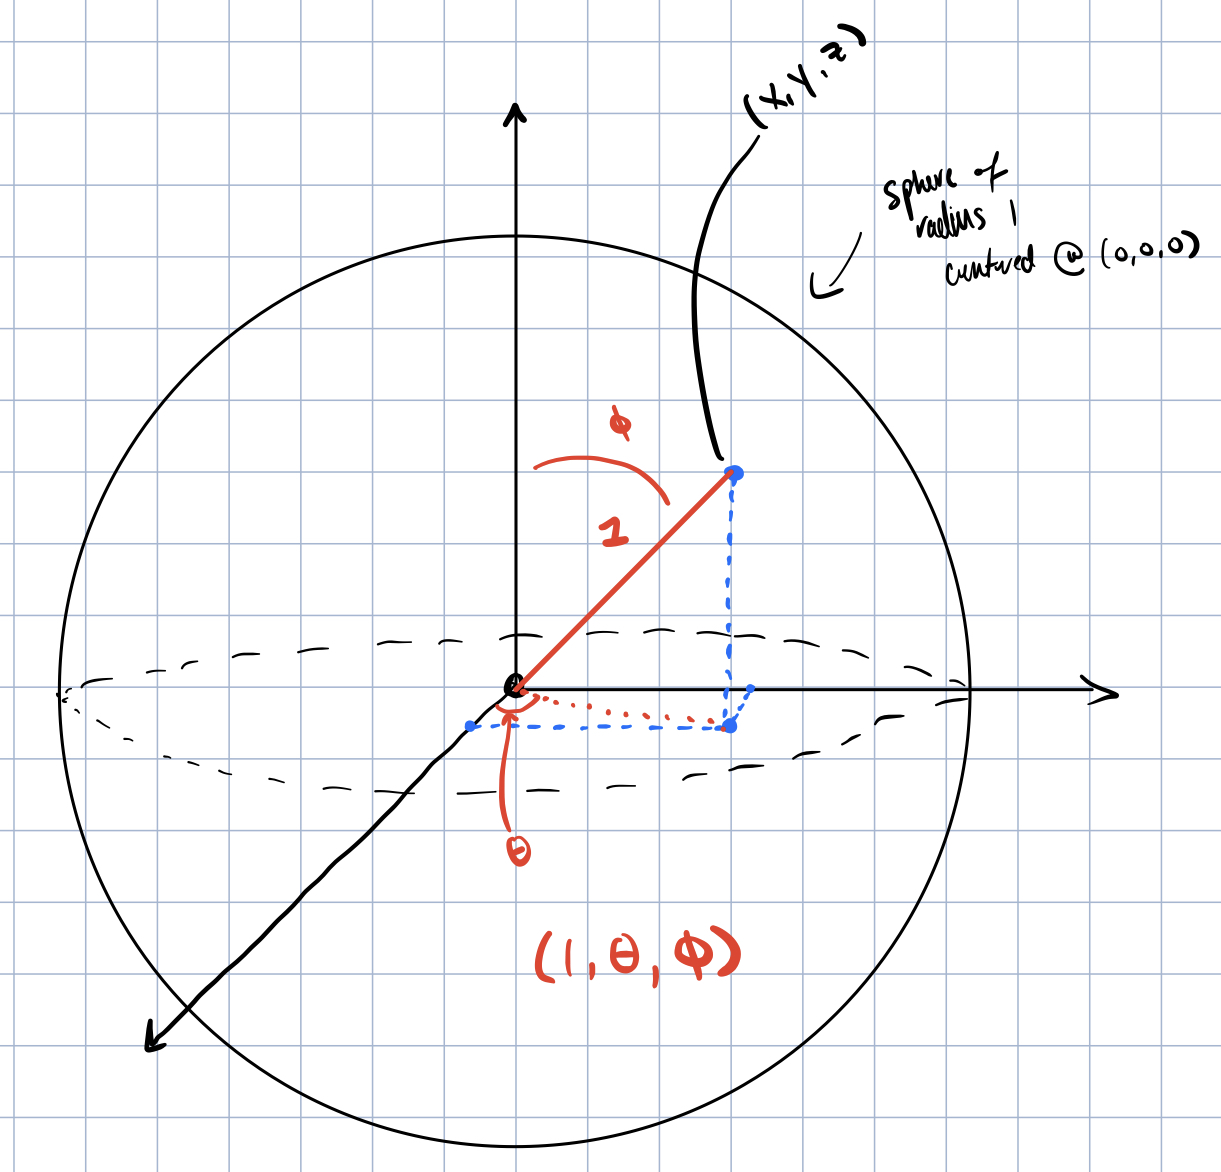
\includegraphics[scale=.3]{bloch}
\end{center}
As you can see, the coordinate system we use for this is $(\underbrace{1}_{\text{Magnitude}},\underbrace{\theta}_{\text{y-axis rotation}},\underbrace{\phi}_{\text{Downward z-direction}})$, as you can see, the highest magnitude of a point is 1, meaning that it lies on the outer rim of the graph, with 100\% of the system "accounted for".  The following two entries in the coordinates will be described in depth as they are much more complicated.
\paragraph{What is $\psi$ when in polar form?} 
\begin{equation}
\begin{split}
\ket{\psi} &= \C^2 \\
\ket{\psi} &= \alpha\ket{0} + \beta\ket{1} \\
\ket{\psi} &= \underbrace{|\alpha| e^{i\gamma_1}}_{\text{Polar form of $\alpha$}}\ket{0}+\underbrace{|\beta| e^{i\gamma_2}}_{\text{Polar form of $\beta$}}\ket{1}\\
\ket{\psi} &= \boxed{\underbrace{e^{i\gamma_1}}_{\text{Global phase shift}}(|\alpha| \ket{0} + |\beta| \underbrace{e^{i(\gamma_2-\gamma_1})}_{\text{Relative phase shift}}}
\end{split}
\end{equation}

\paragraph{What is $\theta, \phi$?} 
Now that we have the polar form of the state vector $\psi$, we can derive what $\theta$ and $\phi$ are.  Let us first define 
\begin{equation}
\underbrace{\theta}_{[0,2\pi]} = \gamma_2 - \gamma_1
\end{equation} 
Simplifying what this math is saying is take the global phase shift, set this as the "perspective", then we can look at how far out of phase our $\beta$ is and choose that as our relative phase shift.  This means we can completely eliminate the imaginary component from $alpha$ as we are setting that vector as the point of view.  Now lets find $\phi$.\\
\\
Find $\underbrace{\phi}_{[0,\pi]}$ such that $(cos(\frac{\phi}{2}), sin(\frac{theta}{2}) = (|\alpha|, |\beta|)$, that means that 
\begin{equation}
\ket{\psi} \underbrace{\approx}_{\text{"Up to a global phase shift"}} cos(\frac{\phi}{2})\ket{0} + sin(\frac{\theta}{2}) e^{i\theta} \ket{1}
\end{equation}

Lets look at an example of what this equation looks like with actual numbers.
\begin{example}
\begin{equation}
\begin{split}
\ket{0} &\rightarrow \alpha = 1, \;\; \beta = 0\\
cos(\frac{\phi}{2}) &= 1 \;\;\;\; sin(\frac{\phi}{2}) = 0\\
&\rightarrow \phi = 0\\
&\rightarrow \theta = 0\\
\ket{0} &\approx (1,0,0)
\end{split}
\end{equation}

\begin{equation}
\begin{split}
\ket{1} &\rightarrow \alpha = 0, \;\; \beta = 1\\
cos(\frac{\phi}{2}) &= 0 \;\;\;\; sin(\frac{\phi}{2}) = 1\\
&\rightarrow \phi = \pi\\
&\rightarrow \theta = 0\\
\ket{0} &\approx (1,0,\pi)
\end{split}
\end{equation}

As you can see in both of these we do not have any theta, that is because these are both pure states, meaning there is no relative phase shift, or more so it does not matter because we are able to get 0 or 1 from the sin and cos, this will change with states that are in some state of superposition, meaning that relative phase shift matters.
\end{example}


Before we move on lets look at what that looks like on the Bloch Sphere:
 \begin{center}
 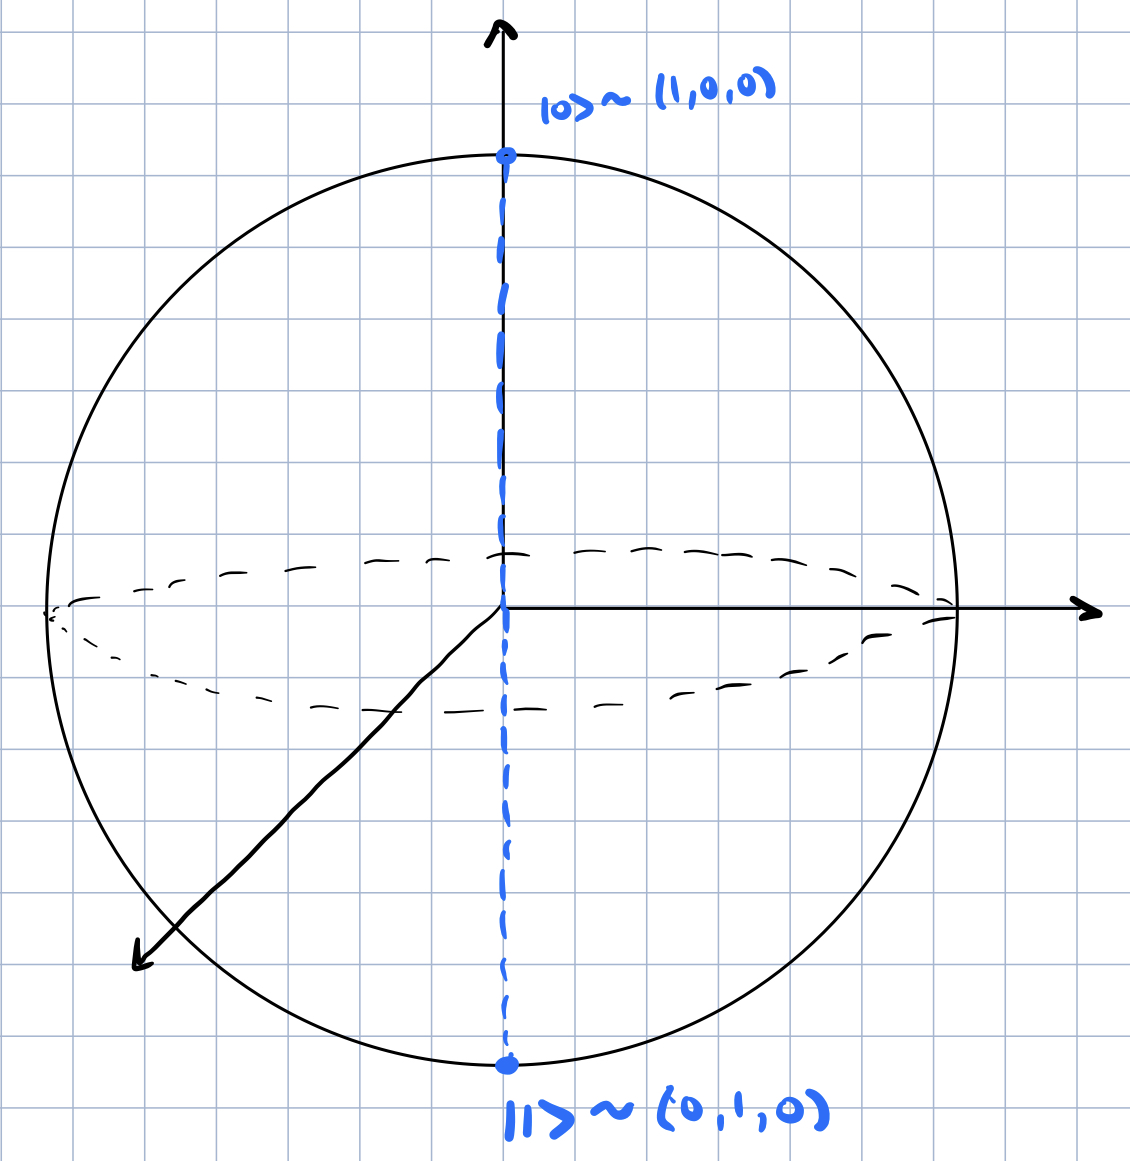
\includegraphics[scale=.3]{0and1}
 \end{center}
 As you can see, they are on the two "north/south" poles on the sphere, further reinforcing why that theta does not matter: because that spin on the y axis would not change how the vector looks! Very interesting!

\pagebreak

\subsection{Quantum Gates}
Well we know what these particles look like, and we know how they are represented, but we still don't know how to do anything with them!  Good thing we are about to learn about quantum gates.  As we mentioned before, these gates are very important with doing things with the particles, more importantly without collapsing them.  Lets get into it.

\subsubsection{Classical Gate Overview}
I have little desire to completely rehash classical logic gates, but in general it is something that changes a 0 to a 1, or swap, or clone. A couple quick examples are below.

\begin{example}
\begin{equation}
\begin{split}
I: 0 \rightarrow 0\\
NOT: 0 \rightarrow 1
\end{split}
\end{equation}
As you can see, the identity passess the value of the bit through, while the not gate flips the value.  This may seem elementary at first but combining these into more complex systems can lead to large and very complex operations.  
\end{example}

\subsubsection{Quantum Gate Introduction}
So real quick let us recall what a quantum gate is, it is just a unitary transformation (i.e. unitary matrices applied to our qubits).  Something interesting is because they are unitary transformations, this means that all of these operations can be reversed.  Lets look at a couple common ones.

\begin{example}
\begin{equation}
\begin{split}
U: \ket{0} &\rightarrow \alpha\ket{0} + \beta\ket{1}\\
\underbrace{\sigma_x = X}_{\text{QNOT}}: \ket{0},\ket{1} &\rightarrow 1\\
-i\sigma_Y = Y =  \ket{0},\ket{1} &\rightarrow \ket{-1},\ket{0} \\
\sigma_z = Z =  \ket{0},\ket{1} &\rightarrow \ket{0},\ket{-1}\\
H =  \ket{0},\ket{1} &\rightarrow \ket{\sigma_x^+},\ket{\sigma_x^-} \\ 
\end{split}
\end{equation}
As you can see we are using the Pauli spin matrices to make these quantum gates, but one of these gates may seem foreign, and rightfully so. "H" is the Hadamard gate, which if you can see, puts the particle into a state of complete superposition.  This is an important gate that is used constantly for this exact purpose.   
\end{example} 


\subsubsection{Common Quantum Gates}
Below is a list of some of the most common quantum gates that are useful in information transmission.\\

QNOT:
\begin{equation}
\begin{split}
QNOT: &\sigma_x\;(X)\; \bmat{0&12\\1&0}\\
	  &\ket{0} \rightarrow \ket{1}\\
	  &\ket{1} \rightarrow \ket{0}\\	  
\end{split}
\end{equation}

The next couple need three bits, two bits that are the inputs, then one bit that is the output based off of the two bits.
\\

QAND:
\begin{equation}
\begin{split}
& \ket{xyz} \rightarrow \bmat{x=y=1,\; \ket{xy \neg z}\\ \text{else } \ket{xyz}}\\
\end{split}
\end{equation}

QOR:
\begin{equation}
\begin{split}
      (I \otimes I \otimes X) * &CNOT * (X \otimes X \otimes I)\\
	  &\ket{00} \rightarrow \ket{00}\\
	  &\ket{01} \rightarrow \ket{01}\\
	  &\ket{10} \rightarrow \ket{11}\\
	  &\ket{11} \rightarrow \ket{10}\\	
\end{split}
\end{equation}

Hadamard:
\begin{equation}
\begin{split}
      &\ket{0} \rightarrow \frac{1}{\sqrt{2}}(\ket{0}+\ket{1})\\
	  &\ket{1} \rightarrow \frac{1}{\sqrt{2}}(\ket{0}-\ket{1})\\	  
\end{split}
\end{equation}





\pagebreak

\subsubsection{Measuring Qubits}
\underline{Recall}: Suppose the single qubit system is in state $\ket{x} = a\ket{0} + b\ket{1}$, find the probability the state is $\ket{0}$ (+1 outcome) or $\ket{1}$ (-1 outcome) upon measurement of $\sigma_z$\\
\underline{Idea}: Let's try and use the spectral projection associated to $\sigma_z = \bmat{1 &0\\ 0 &-1}$:
\begin{equation}
\begin{split}
= 1\underbrace{\ket{0}\bra{0}}_{M_0} + (-1)\underbrace{\ket{1}\bra{1}}_{M_1}\\
p(0) = a^2 = \bra{x}M_0\ket{x}\\
p(1) = b^2 = \bra{x}M_1\ket{x}\\
\end{split}
\end{equation}

\subsubsection{Applying quantum measurements}
\paragraph{BB84 Protocol - Quantum Key Distributions}
One of the most prevalent aspects of quantum information currently is through quantum encryption.  The aspect of collapse makes this it impossible for someone to eavesdrop, more on that in the chapter.  For a quick introduction into quantum key distribution, lets look at a protocol developed in 1984, muich before there was a single quantum computer even beginning to be built.  Anyways, lets get into it, let us visualize what a typical communication looks like.
\\
\\
\begin{center}
 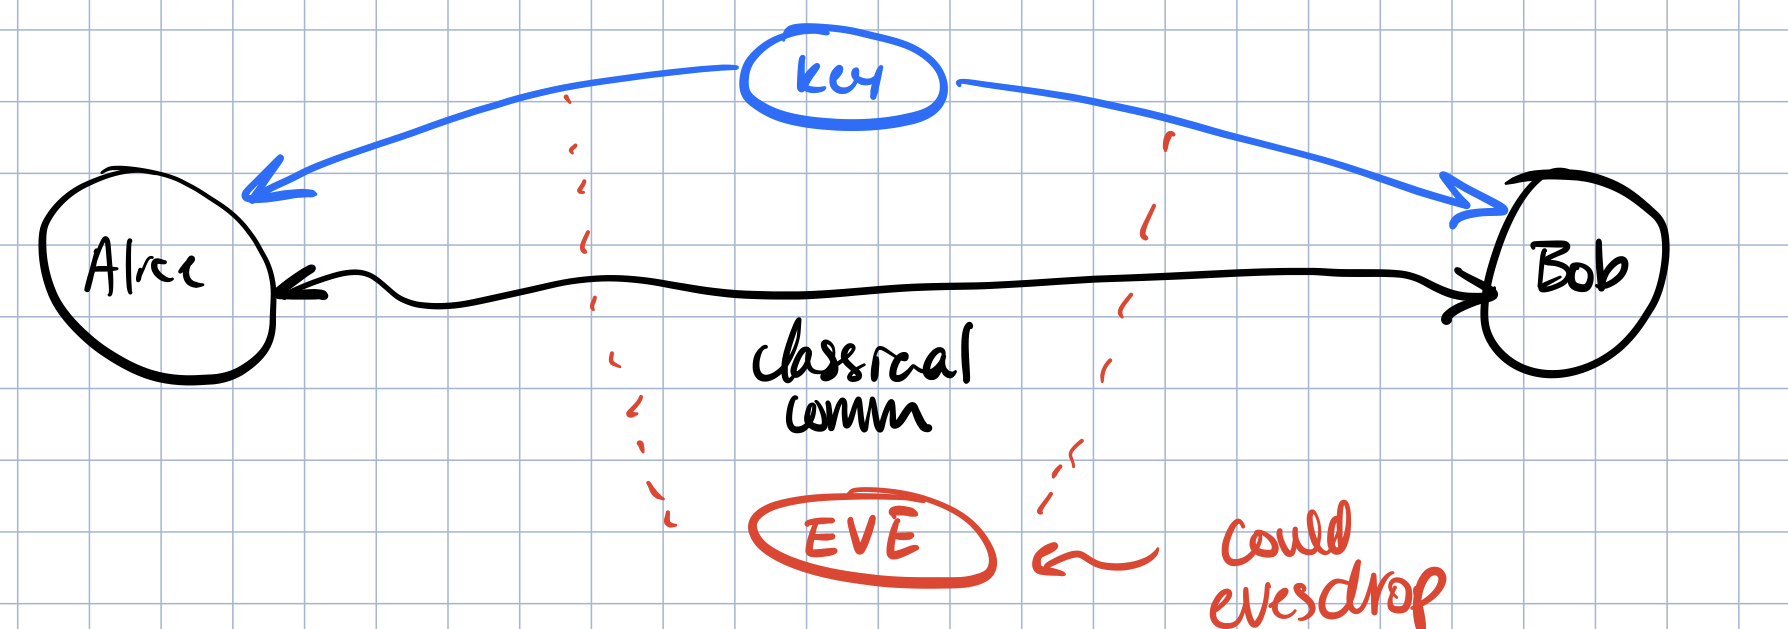
\includegraphics[scale=.3]{aandb}
\end{center}

We will be using a \textbf{one time pad}, meaning when we get the key we will apply it to our data, flipping bits if it is a one and leaving it the same if not.  Now we can set up the problem.

\begin{itemize}
\item First, over the classical channel, Alice will communicate to Bob what basis they will be preparing the particles with.  
\item Bob and Alice then take the stream of qubits (in superposition) and measure each measure them with random basis.  
\item Next, Bob tells Alice which basis he used to measure all of the different qubits, and if they did not choose the same, Alice secretly throws out those qubits because no information can be gleaned from them.
\item In the end we should have $\approx N/2$ good qubits (meaning w.r.t. the same basis, 50\% chance.)
\item If no one was listening, this is it, Alice chooses some number of those good qubits, as they both have the same values as those qubits are entangled, and use that as the one time pad key.  
\end{itemize}
This can seem easy enough, and as long as there is no outside person listening this seems fine.  Even if someone was listening, lets say for example on the classical channel, they would not be able to do anything with the information because they never dicuss the outcome of any of the particles.  Eve actually can't even listen on the quantum channel where the information is being sent because if she made a measurement, the particle would collapse!  That means that to make this impossible, like actually mathematically impossible to crack, we need to detect that someone is collapsing the particles.

\paragraph{Detecting collapse, tampering with information}
To check that someone is listening we will have to sacrifice a certain numbers of our above "good" qubits to check the outcome value to make sure no one collapsed the value and sent the particle on again.  If eve collapsed the particle, the value that Bob reads will differ from what Alice reads.  Alice will choose bits at random and check values, and if there are more than $\frac{N}{4}$ bits, we must retransmit because someone was listening in.  A quick matrix of what this would look like is below.
\\
\\
\begin{center}
 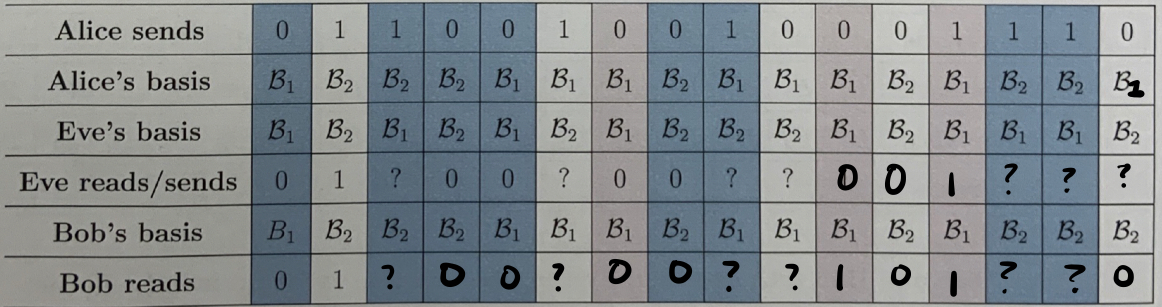
\includegraphics[scale=.3]{eve}
\end{center}

As you can see, when Eve measures, Bob receives a 0 even though Alice received a one and vice versa.  These are the bits that are detected in tamper investigation.  \\
\\
Apologies for the slightly abbreviated version of this, this is very in depth and many mathematic concepts at play, but I realistically do not have time to spend writing all of those equations down. Please show me mercy.    

\pagebreak

\subsection{Quantum Gates as Density Matrices}
Something that is always a problem when it comes to quantum information transmission is reliability.  When you are working at the atomic and sometimes subatomic particles, you have to be extremely precise.  What happens if there is any level of noise or inaccuracy in the bits.  Will the quantum logic still apply to the particles?  This is where quantum gates being represented as density martices comes in.  
\begin{example}
Suppose we want to send $\ket{11}$ as $\ket{11}$ by applying a CNOT.  80\% of the time $\ket{11}$ is sent, 15\% of the time $(H \otimes I) \ket{10}$ is sent, and 5\% of the time $(H \otimes H)CNOT(H \otimes H)$ is sent.  This means that the vector received is
\begin{equation}
0.80CNOT\ket{10} + .15(H \otimes I)\ket{10} + 0.05 CNOT' \ket{10} 
\end{equation}
This can be represented in a much simpler manner using density matrices, to do this we must apply some quantum gate U to a vector.  This gives us $\psi \rightarrow U\psi$.
\begin{theorem} If $\rho$ is a pure state density matrix $\rho = \ket{\psi}\bra{\psi}$ for some $\ket{\psi} \in \C^n$, 
\begin{equation}
\rho = \ket{\psi}\bra{\psi} \rightarrow (u\ket{\psi})(u\ket{psi})^\dagger = U\ket{\psi}\bra{\psi}U^\dagger = U\rho U^\dagger
\end{equation}
\end{theorem}
\end{example}
\pagebreak

\section{Conclusion and Parting Words}
Thank you for spending the time to read through this document, I realize that this may not be the best document by any stretch, and there is still lots of work to make this actually useful to someone who wants to learn, but taking into account that this was completed in tandem with two jobs and developing a satellite, I am actually somewhat satisfied.  Overall, this is a field that is just barely blooming, and this is the math and concepts that are necessary to even begin to comprehend the new research being done in this field.  Please take as much as possible from this, and have as much fun with this as I did in the semester I took this class.  Goodbye! 


\end{document}

